\documentclass[11pt,twoside,openright]{report}
\usepackage[a4paper,width=155mm, inner=25mm, top=30mm,bottom=40mm, marginparsep=0mm]{geometry}
\usepackage[utf8]{inputenc} 
\usepackage[T1]{fontenc} 
\usepackage{longtable}
\usepackage[czech]{babel} 
\usepackage{graphicx}
\usepackage{emptypage} % maže číslování na prázdných stranách
\usepackage[numbers,sort&compress]{natbib}
\usepackage{formatting,amsfonts,amsmath,amssymb}
\usepackage{booktabs,mathtools}
\usepackage{lipsum,url}
\usepackage[unicode]{hyperref}
\usepackage{textcomp}
\usepackage{multirow}
\usepackage{setspace}
\usepackage{array}
\usepackage{float}
\usepackage{mwe}
\usepackage{appendix}
\usepackage{pdfpages}
\usepackage{etoolbox}
\usepackage[nottoc]{tocbibind}
\usepackage{tikz}
%\usepackage{enumerate}
\usepackage{enumitem}
\usepackage{algorithmic}
\usepackage{algorithm}
\usepackage{csquotes}
\usetikzlibrary{shapes, arrows.meta}
\usetikzlibrary{backgrounds,calc}
\DeclarePairedDelimiter{\ceil}{\lceil}{\rceil}
\BeforeBeginEnvironment{appendices}{\gdef\thechapter{\ }}
\AtBeginEnvironment{appendices}{\renewcommand\thesection{\Alph{section}}}

% \cmidrule have problem with Czech
\usepackage{regexpatch}
\makeatletter
% Change the `-` delimiter to an active character
\xpatchparametertext\@@@cmidrule{-}{\cA-}{}{}
\xpatchparametertext\@cline{-}{\cA-}{}{}
\makeatother

%\usepackage[nottoc,numbib]{tocbibind}
\usepackage{fancyhdr}
\usepackage{booktabs}
\usepackage{subfig}
\usepackage{fancybox}

\DeclarePairedDelimiter\abs{\lvert}{\rvert}%
\DeclarePairedDelimiter\norm{\lVert}{\rVert}%
\makeatletter
\renewcommand{\ALG@name}{Algoritmus}
\makeatother
\pagestyle{fancy}
%\renewcommand{\chaptermark}[1]{%
%  \markboth{\MakeUppercase{\thechapter\ \quad  #1}}{}% 
%}
\renewcommand{\chaptermark}[1]{%
  \markboth{\MakeUppercase{#1}}{}% 
}
\fancyfoot{}{}{}
\fancyhead[LO,LE]{}
\fancyhead[RO]{\leftmark}
\fancyhead[RE]{}
\fancyfoot[RO]{\vspace*{0.8\baselineskip}\thepage}
\fancyfoot[LE]{\vspace*{0.8\baselineskip}\thepage}
\renewcommand{\headrulewidth}{0pt}
\renewcommand{\footrulewidth}{0pt}

\fancypagestyle{plain}{%
\fancyhead[RO]{}
\fancyhead[LO,LE]{}
\fancyfoot[RO]{\vspace*{0.8\baselineskip}\thepage}
\fancyfoot[LE]{\vspace*{0.8\baselineskip}\thepage}
\renewcommand{\headrulewidth}{0pt}
\renewcommand{\footrulewidth}{0pt}
}
\makeatletter
\renewcommand\@dotsep{300}   % default value 4.5
\makeatother

\linespread{1.25}
\let\cleardoublepage=\clearpage
\begin{document}
\pagenumbering{gobble}

\cleardoublepage
\thispagestyle{empty}
%\thisfancypage{\setlength{\fboxsep}{5pt}\doublebox}{}
%\setlength\intextsep{0mm}
\noindent

\includegraphics[width=0.45\textwidth]{IMG/TOP/logoVSCHT_zakl_CB.png} \\
\vspace{10mm}
\\
{\Large \textbf{Fakulta  chemicko-inženýrská}
\\ [5mm]
Ústav počítačové a řídicí techniky}

\vspace{30mm}


\begin{spacing}{0.9}
\Huge\noindent POUŽITÍ ADAPTIVNÍCH SYSTÉMŮ PŘI ANALÝZE DAT\\ 
\end{spacing}
\vspace{20mm}

\noindent
{\Large \textbf{TEZE DISERTAČNÍ PRÁCE}} 

\vspace{10mm}

\begin{table}[!h]
\begin{tabular}{  l l |l  l }
\hspace{-0.5em}AUTOR & \hspace{0mm} & & {\Large \textbf{Ing. Jan Vrba}} \\ [5mm]
\hspace{-0.5em}ŠKOLITEL &  &  & \textbf{\large doc. Ing. Jan Mareš, Ph.D.}\\ [5mm]
\hspace{-0.5em}ŠKOLITEL  SPECIALISTA             &     &   & {\textbf{\large doc. Ing. Pavel Hrnčiřík, Ph.D. }} \\ [5mm]
\hspace{-0.5em}STUDIJNÍ PROGRAM &  &  & {\large Chemické a procesní inženýrství (čtyřleté)} \\ [5mm]
\hspace{-0.5em}STUDIJNÍ OBOR    & &   & {\large Technická kybernetika}\\ [5mm]
\hspace{-0.5em}ROK          &       &   & \textbf{2020} 
\end{tabular}


\end{table}

%%====================================================Declaration=====================
%\newpage
%\thispagestyle{empty}
%\vphantom{a}
%\vspace{13cm}
%\begin{figure}[H]
%\pdfimageresolution=133 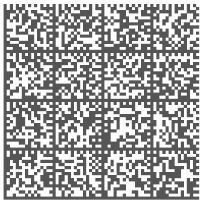
\includegraphics{IMG/TOP/QR.png}
%\end{figure}
\cleardoublepage
\thispagestyle{empty}\

\newpage
 




%-------------------------------Abstract CZ ---------------------------------------------
\clearpage
\thispagestyle{empty}
%-------------------------------Abstract CZ ---------------------------------------------

\noindent {\bf \large Souhrn} \\ [5mm]
Dizertační práce se zabývá použitím adaptivních systémů v oblasti detekce novosti. Tento přístup v oblasti detekce novosti v datech se stal v posledních letech slibným směrem výzkumu. V rámci této práce je navržen nový algoritmus pojmenovaný jako Extreme Seeking Entropy. Tento algoritmus je založen na vyhodnocování přírůstku adaptivních parametrů systémů pomocí zobecněného Paretova rozdělení. Navržený algoritmus byl otestován na celé řadě typů syntetických dat, která reprezentují různé druhy novosti. Pro detekci změny trendu a skokové změny generátoru signálu pak bylo provedeno i vyhodnocení úspěšnosti detekce. Dále byla provedena experimentální studie zabývající se časovou náročností výpočtu algoritmu, vyhodnocena ROC (Receiver Operating Characteristic) křivka pro detekci změny trendu, a provedena studie detekce epilepsie v záznamu EEG myši.\\ [5mm]
\noindent {\bf \large Klíčová slova}  \\ [5mm] \noindent {\it adaptivní systémy, detekce novosti, časové řady, extreme seeking entropy} \\ [5mm]

\noindent {\bf \large Summary} \\ [5mm] 
The dissertation deals with the use of adaptive systems in the field of novelty detection. The use of adaptive systems for detecting novelty in data has become a promising direction of research in recent years. In this work, a new algorithm was designed using adaptive systems, called Extreme Seeking Entropy. This algorithm is based on evaluating the increment of adaptive parameters of systems using a generalized Pareto distribution. The proposed algorithm has been tested on a number of types of synthetic data that represent different types of novelty. To detect a change in the trend and a step-change in the signal generator, an evaluation of the detection success was performed. Furthermore, an experimental study was performed dealing with the time consumption of the algorithm, the ROC curve was evaluated to detect a change in the trend, and a study was performed to detect epilepsy in the EEG mouse record.
\\ [5mm]



\noindent {\bf \large Keywords}  \\ [5mm]
{\it adaptive systems, novelty detection, time series, extreme seeking entropy}

\cleardoublepage
\thispagestyle{empty}








%%v~v~v~v~v~v~v~v~v~v~v~v~v~v~v~v~v~v~v~v~v~v~v~v~v~v~v~v~v
%\thispagestyle{empty}
%%v~v~v~v~v~v~v~v~v~v~v~v~v~v~v~v~v~v~v~v~v~v~v~v~v~v~v~v~v

\tableofcontents

%\addtocontents{toc}{~\hfill\textbf{Page}\par}
%\addcontentsline{toc}{chapter}{Contents}
%%v~v~v~v~v~v~v~v~v~v~v~v~v~v~v~v~v~v~v~v~v~v~v~v~v~v~v~v~v

%\newpage
%\setcounter{page}{1}

% TAK AT TO JDE OD RUKY


\chapter{Úvod}
\pagenumbering{arabic}
\setcounter{page}{1}

Tato disertační práce je věnována problematice využití adaptivních systémů při analýze dat. Vzhledem k exponenciálnímu celosvětovému nárůstu objemu dat \cite{expo} a ke zvyšování jejich variability roste i potřeba tato data analyzovat, kategorizovat a vytěžovat. Analýzou dat rozumíme proces, kdy z nezpracovaných naměřených dat získáme nějakou interpretovatelnou informaci, s kterou pak lze dále pracovat. Jedna z možných důležitých interpretací nově získaných dat je, zda-li se nově získaná data nějakým zásadním způsobem odlišují od předchozích dat. Této problematice se věnuje obor detekce novosti, neboli anomálií, který spadá do oblasti vytěžování dat a strojového učení. Úspěšná detekce novosti pak může být využita k vícero účelům. Například k diagnostice sledovaného procesu, ke změně struktury nebo parametrů adaptivního modelu za účelem zlepšení predikce, z konkrétních aplikací pak k odhalení neoprávněného vniknutí do sítě nebo zneužití dat, v lékařství se detekce novosti používá k diagnostickým účelům, z průmyslových aplikací pak k detekci poruchy a monitoringu stavu strojů, senzorů, ve zpracování textových dat k detekci nových témat, originálnosti textů atd. Spektrum využití je velice široké.
\par
V oblasti detekce novosti byla v posledních desetiletích intenzivního vývoje navrhnuta celá řada algoritmů. Vzhledem k rostoucímu výpočetnímu výkonu a rozmanitosti analyzovaných dat rostla i potřeba nových algoritmů. Nové algoritmy typicky předčily ostatní v rámci jedné aplikace, respektive v rámci jednoho typu dat.  Doposud se však nepodařilo vytvořit algoritmus, který by ve všech (nebo alespoň ve významné části) oblastech použití předčil již publikované algoritmy. I proto vznikají v oblasti detekce novosti neustále nové přístupy, které navíc umožňují analyzovat nové typy dat.

\section{Cíle dizertační práce}\label{chap:cile}
Cíle předkládané dizertační práce jsou:
\begin{enumerate}[label=\textbf{\arabic*})]
\item \textbf{Návrh algoritmu pro detekci novosti v datech s využitím adaptivních systémů}
\par 
Navrhovaný algoritmus pro detekci novosti bude využívat adaptivní systémy a bude mít interpretovatelný výstup. Jeho použití by mělo být možné v kombinaci libovolným adaptivním systémem. Algoritmus bude implementován v jazyce Python, který je v současné době jedním z nejrozšířenějších programovacích jazyků.
\item \textbf{Otestování navrženého algoritmu na syntetických datech}
\par 
Navržený algoritmus bude otestován na syntetických datech, která budou simulovat různé typy novosti a budou obsahovat šum. Mezi testovanými daty budou i data časových řad obsahujících trend. Výsledky algoritmu budou porovnány se obdobnými soudobými metodami využívajícími adaptivní systémy, konkrétně s algoritmem Learning Entropy a Error and Learning Based Novelty Detection.
\item \textbf{Provedení případových studií na reálných datech z oblasti biomedicíny a chemie}
\par 
Pro otestování navrženého algoritmu je zásadní provedení případových studiích na reálných datech. 
\item \textbf{Vyhodnocení kvality navrženého algoritmu z pohledu úspěšnosti detekce novosti} \par
Pro vyhodnocení kvality navrženého algoritmu budou určeny dosažené přesnosti detekce v různých scénářích. Dále budou pro vybrané scénáře určeny ROC křivky a vyhodnocena plocha pod nimi. Vyhodnocení bude provedeno pro scénáře s různými poměry signál-šum. Výsledky budou porovnány s výsledky algoritmů Learning Entropy a Error and Learning Based Novelty Detection. 

\end{enumerate}


\chapter{Algoritmus Extreme Seeking Entropy}\label{chap:ese}
V této kapitole je představen algoritmus pro detekci novosti nazvaný Extreme Seeking Entropy (ESE), který tvoří hlavní teoretický výsledek předkládané dizertační práce (publikováno v \ref{ese_mdpi}). Navržený algoritmus, vychází z předpokladu, že novost v datech se projeví neobvykle velkými přírůstky vah adaptivního filtru, který danou řadu dat modeluje.
\par Nejprve uvažujme myšlenkový experiment, ve kterém máme dokonale nastavený adaptivní filtr, jehož chyba predikce $e$ je nulová pro všechny vstupní hodnoty. Potom přírůstky adaptivních vah tohoto filtru budou nulové. V případě, že dojde k nějaké změně v generátoru dat pro tento filtr, začne se filtr opět adaptovat což vyústí v nenulové změny adaptivních vah, které budou reflektovat novost způsobenou změnou vlastností daného generátoru.
\par
V publikacích \cite{ivoLE1,ivoLE2}, kde autoři představují algoritmus Learning Entropy, je zmíněna obecná míra snahy adaptivního filtru o adaptaci, $L$, která slouží k vyhodnocení neobvykle velkých přírůstků adaptivních vah a je definovaná jako
\begin{equation}
L(k)=A(f(\Delta \textbf{w})))
\end{equation}
kde $A$ je obecně nějaká agregační funkce a funkce $f$ je funkce která nějakým způsobem kvantifikuje odchylku v adaptaci adaptivních parametrů filtru.

\par
Nejprve uvažujme, že hodnota funkce $f$, která slouží k vyhodnocení neobvykle velkých přírůstků by měla mít neobvykle velkou (nebo neobvykle malou) hodnotu v okamžiku, kdy přírůstky adaptivních vah filtru $\Delta \textbf{w}$ jsou neobvykle velké. Dalším požadavkem je, aby tato funkce zohledňovala i nějakou historii těchto přírůstků. Přirozeně se tedy nabízí nějaká  vhodná distribuční funkce $f_{cdf}$. S ohledem na požadavek, že neobvykle velké přírůstky vah by měli být reflektovány neobvykle velkou hodnotou míry snahy o adaptaci, nabízí se jako vhodná funkce $A$, kterou uvažujeme ve tvaru
\begin{equation} \label{eq:ND_score}
A(f(\Delta \abs{\textbf{w}}(k)) = -\log \prod_{i=1}^n(1 - f_{{cdf}_i}(\lvert \Delta  w_i(k)\rvert)).
\end{equation}
Uvedená agregační funkce $A$ má pro neobvykle velké přírůstky vah neobvykle velkou kladnou hodnotu, pokud jsou hodnoty $f_{cdf}$ blízké 1. Člen $1-f_{cdf}$ je vlastně komplementární distribuční funkcí (funkce přežití, spolehlivostní funkce). Výhodou uvedeného přístupu je absence potřeby nastavovat několik prahů pro detekci.
\par 
Jak již bylo uvedeno, cílem je tedy vyhodnotit neobvykle velké přírůstky vah adaptivního systém. Nejprve je nutné určit nějaký práh $z$, podle kterého můžeme přírůstky adaptivních vah filtru rozdělit do dvou množin. Množinu, která bude obsahovat přírůstky menší než je zvolený práh $z$ označíme $L$. Přírůstek, který je větší nebo roven hodnotě prahu $z$ označíme $H$.  Uvažujme, že obě množiny existují pro každou adaptivní váhu, potom pro $i$-tou adaptivní váhu zvolíme práh $z_i$ tak, že velikosti přírůstku této váhy náleží do jedné ze dvou množin, tak, že:
\begin{equation}
\forall \abs{\Delta w_i} < z_i \in L_i
\end{equation}
\begin{equation}
\forall \abs{\Delta w_i} \geq z_i \in H_i
\end{equation}
Vzhledem k výše zmíněnému předpokladu o velikosti změn vah adaptivního filtru a novosti v datech, uvažujme, že přírůstky náležející množině $L_i$ pravděpodobně neobsahují informaci o novosti během adaptace, a proto nebudou vyhodnocovány. Množina $H_i$ by měla obsahovat přírůstky adaptivních vah filtru, u kterých lze očekávat, že mohou nést nějakou informaci o novosti v datech.
\par
Nyní můžeme zavést novou míru, kterou nazvěme Extreme Seeking Entropy (ESE), definovanou jako

\begin{equation}\label{eq:ese}
ESE(\abs{\Delta \textbf{w}(k)})=-\log \prod_{i=1}^{n_w}(1-f_{cdf_i}(\abs{\Delta w_i(k)}))
\end{equation}
kde
\begin{equation}
  f_{cdf_i}(|\Delta w_i(k)|)=\begin{cases}
    0,\, |\Delta w_i(k)| \in L_i \\
    F_{(\xi_i,\mu_i,\sigma_i)}(|\Delta w_i(k)|),\, |\Delta w_i(k)| \in H_i.
  \end{cases}
\end{equation}
a funkce $F_{(\xi_i,\mu_i,\sigma_i)}$ je distribuční funkce zobecněného Paretova rozdělení (GPD). Přírůstky adaptivních vah, které jsou menší než hodnota prahu $z$ získaného metodou Peak-Over-Threshold, nezmění hodnotu $ESE$. Přírůstky vah, které mají velice malou pravděpodobnost a spíše nesou nějakou informaci o novosti v datech, způsobí velký nárůst hodnoty $ESE$. Zásadním aspektem navrhovaného algoritmu je, že mohou být vyhodnocovány buď všechny získané přírůstky vah, anebo lze vyhodnocovat pouze nejnovějších $n_s$ vzorků a na ně aplikovat metodu POT. Novost potom můžeme vnímat v kontextu těchto $n_s$ vzorků. 
\par
Navrhovaný algoritmus pro detekci novosti v datech je popsán následujícím pseudokódem.

\begin{algorithm}[H]
\caption{Extreme Seeking Entropy}
\begin{algorithmic}[1]\onehalfspacing
\STATE  nastavení $n_s$ a výběr metody POT
\STATE počáteční nastavení parametrů $\xi_i$, $\mu_i$, $\sigma_i$ GPD pro každý adaptivní parametr
\FOR{vzorek $y(k)$}
\STATE výpočet změny adaptivních parametrů filtru $\Delta \textbf{w}(k)$
\STATE aplikace metody POT
\IF{$|\Delta w_i|(k) \in H_i$}
\STATE výpočet parametrů $\xi_i$, $\mu_i$, $\sigma_i$ pro příslušné GPD
\ENDIF
\STATE výpočet hodnoty $ESE$ podle rovnice \ref{eq:ese}
\ENDFOR
\end{algorithmic}
\end{algorithm}

Výhodou navrhovaného algoritmu je, že jediným volitelným parametrem je parametr $n_s$, který ale v případě potřeby můžeme vynechat a zpracovávat všechny historicky dostupné přírůstky adaptivních parametrů. Dále je nutné zvolit vhodnou metodu POT.
\par
Určitou limitací uvedeného algoritmu je, že pro získání první hodnoty $ESE$ potřebujeme nějakou apriorní informaci o parametrech GPD rozdělení. Konkrétněji, pro každou $i$-tou adaptivní váhu musíme mít k dispozici odhad parametrů $\xi_i$, $\mu_i$, $\sigma_i$. Vzhledem k tomu, že adaptivní filtr má $n_w$ různých adaptivních vah, potřebujeme získat odhad $3\cdot n_w$ parametrů aby začal algoritmus ESE poskytovat první hodnoty. Pokud není k dispozici žádná apriorní informace o hodnotách těchto parametrů, potřebujeme získat alespoň $n_s$ vzorků, na jejichž základě můžeme získat první hodnotu $ESE$. Dalším úskalím je proměnlivost parametrů nebo typu rozdělení pravděpodobnosti přírůstků adaptivních vah v čase.
\chapter{Výsledky detekce novosti algoritmem Extreme Seeking Entropy}\label{chap:vysledky}
V dalším textu jsou shrnuty výsledky algoritmu Extreme Seeking Entropy, kterých bylo v rámci práce na dizertační práci dosaženo. Výsledky použití ESE pro detekci pertubace v chaotické časové řadě Mackey-Glass je uvedena v podkapitole \ref{chap:mdpi_mg}. Dále jsou uvedeny výsledky pro: detekci změny rozptylu šumu v náhodném datovém toku (podkapitola \ref{chap:mdpi_noise_change}), detekci skokové změny parametrů generátoru signálu (podkapitola \ref{chap:mdpi_stepchange}), detekci náhle absence šumu (podkapitola \ref{chap:mdpi_noise_ext}), detekci změny trendu (podkapitola \ref{chap:mdpi_trendchange}) a detekci epilepsie v záznamu myšího EEG (viz podkapitola \ref{chap:mdpi_eeg}). Dále jsou uvedeny výsledky vyhodnocení úspěšnosti detekce skokové změny parametrů generátoru signálu (podkapitola \ref{chap:mdpi_step_stats}) a úspěšnosti detekce skokové změny trendu (podkapitola \ref{chap:mdpi_trendchange_evaluation}). V posledních dvou kapitolách je potom vyhodnocení ROC křivky (receiver operating characteristic) pro detekci změny trendu (podkapitola \ref{chap:appel_roc}) a experimentální vyhodnocení výpočetní náročnosti metod odhadu parametrů zobecněného Paretova rozdělení (podkapitola \ref{chap:appel_gpd}).
\par Výsledky v podkapitolách \ref{chap:mdpi_mg}-\ref{chap:mdpi_trendchange_evaluation} byly publikovány v \ref{ese_mdpi}. Výsledky v podkapitolách \ref{chap:appel_roc} a \ref{chap:appel_gpd} pak v publikacích \ref{appel2},\ref{appel3}.

\section{Chaotická časová řada Mackey-Glass a detekce pertubace}\label{chap:mdpi_mg}
Tento experiment byl proveden pro porovnání s výsledky uvedenými v publikaci \cite{ivoLE1}, která je první publikací o algoritmu Learning Entropy. Experiment spočívá v detekci pertubovaného vzorku v chaotické časové řadě, která je výsledkem řešení Mackey-Glassovy rovnice \cite{mackey}.
\begin{equation}
    \frac{dy(t)}{dt}= \beta \cdot \frac{ y(t-\tau)}{1 + y^\alpha(t-\tau)} - \gamma y(t)
\end{equation}
přičemž parametry $\alpha = 10$, $\beta = 0.2$, $\gamma = 0.1$ and $\tau = 17$ byly vybrány tak, aby řešením této rovnice byla chaotická časová řada. Celkem bylo vygenerováno 701 vzorků. Data v diskrétní časový okamžiku $k=523$ pak byly pertubovány podle následujícího předpisu.
\begin{equation}
    y(523) = y(523) + 0.05 \cdot y(523)
\end{equation}
Výsledná časová řada a detail pertubace je znázorněn na obrázku \ref{fig:mackey_details}. Výstup adaptivního filtru a chyba predikce jsou znázorněny na obrázku \ref{fig:mackey_results}. Výsledky metod detekce novosti jsou zobrazeny na obrázku \ref{fig:mackey_results_nd}. Z obrázku je patrné, že globální maximum průběhu $ESE$ odpovídá pertubovaným datům. Globální maximum metod $ELBND$ a $LE$ odpovídá vzorku u něhož byla největší chyba predikce.
\begin{figure}[!ht]
    \centering
    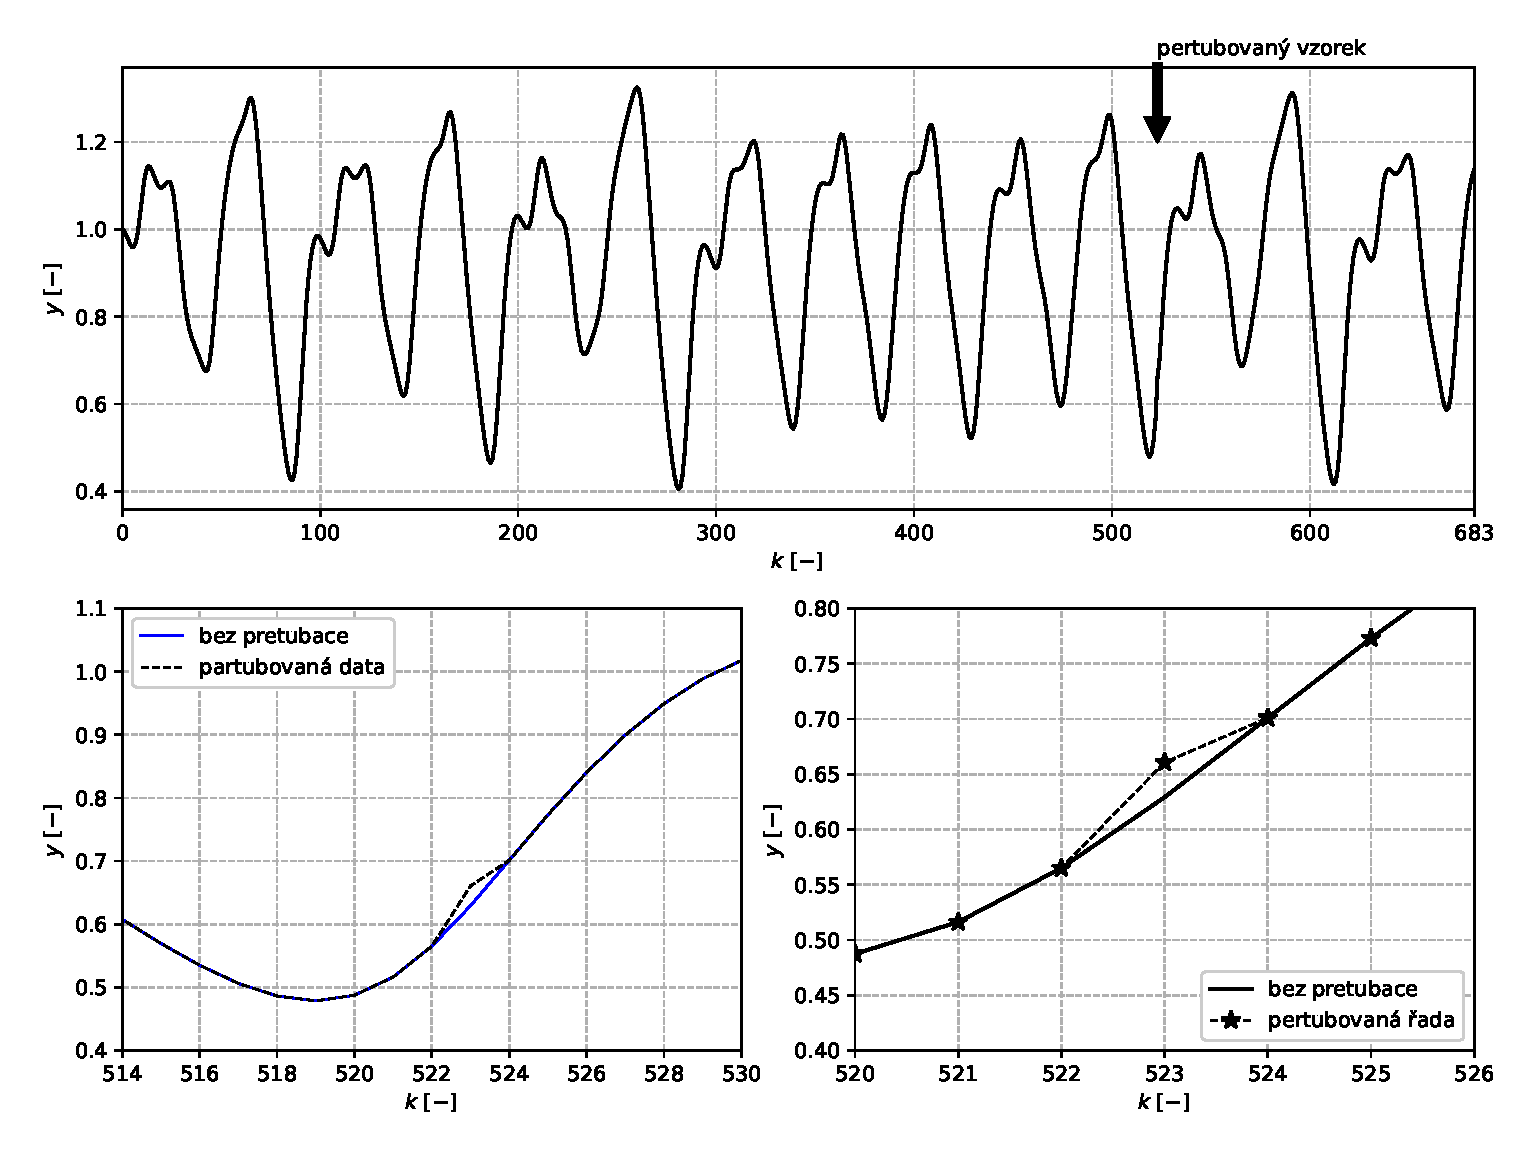
\includegraphics[scale=0.56]{IMG/mdpi/mackeydetails_diz.eps}
    \caption{Horní graf zobrazuje celou datovou řadu. Spodní grafy zobrazují detail pertubovaného vzorku v diskrétní časový okamžik $k=523$.}
    \label{fig:mackey_details}
\end{figure}
\begin{figure}[!ht]
    \centering
    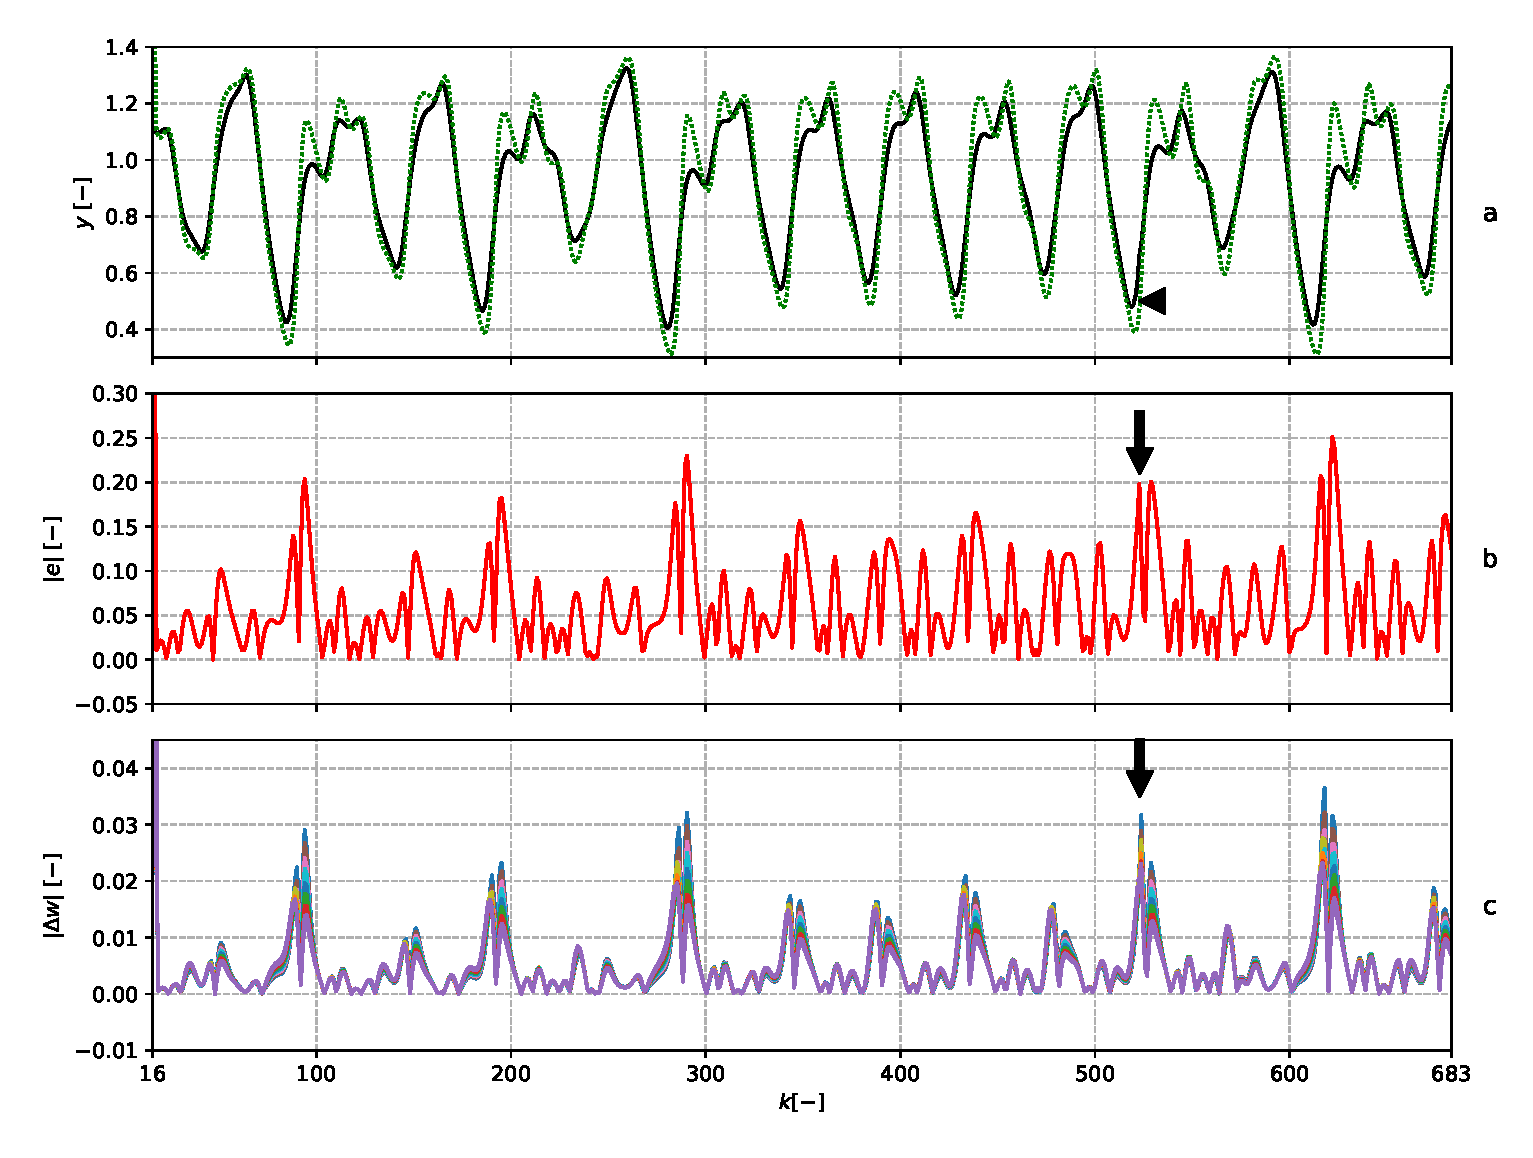
\includegraphics[scale=0.56]{IMG/mdpi/mackey_results.eps}
    \caption{Graf (a) zobrazuje datovou řadu s pertubací (černá plná čára) a výstup adaptivního filtru (tečkovaná zelená čára). Pertubovaný vzorek je označen černou šipkou. Graf (b) zobrazuje velikost chyby predikce $e$ (resp. její absolutní hodnotu). Na grafu (c) jsou znázorněny přírůstky adaptivních vah filtru (resp. absolutní hodnotu těchto přírůstků).}
    \label{fig:mackey_results}
\end{figure}

\begin{figure}[!ht]
    \centering
    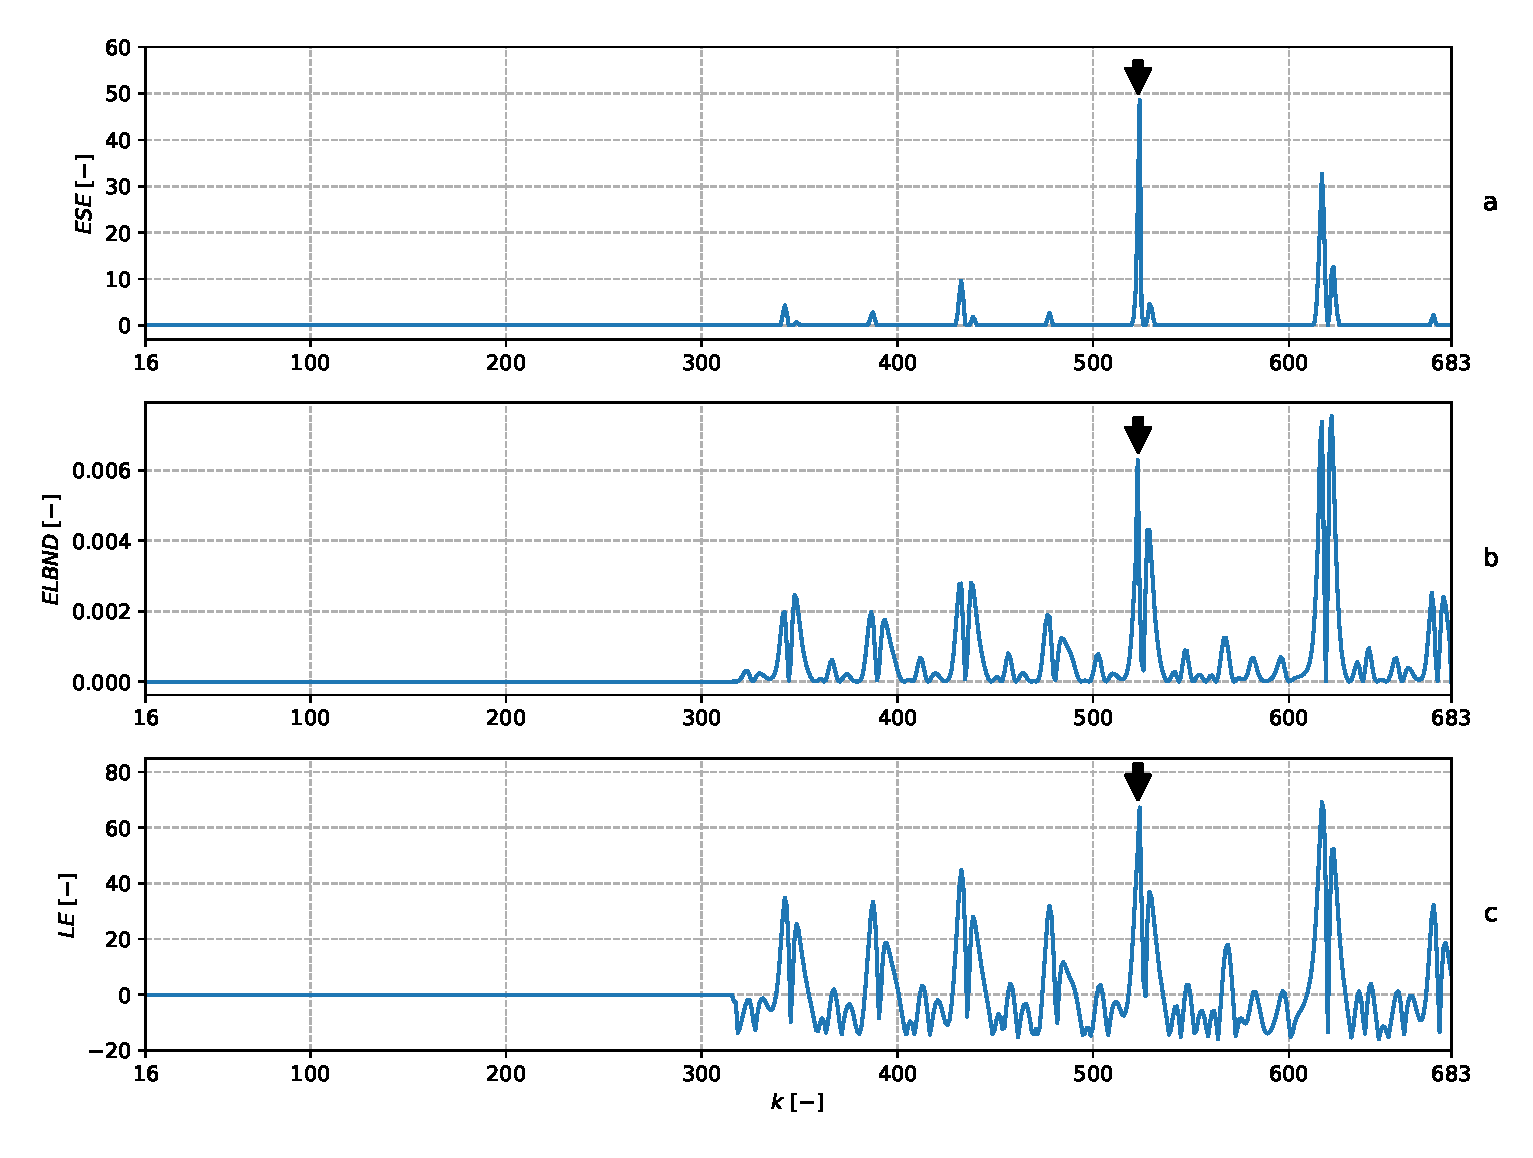
\includegraphics[scale=0.57]{IMG/mdpi/mackey_results_nd.eps}
    \caption{Graf (a) zobrazuje hodnotu ESE. Prvních 300 vzorků je hodnota ESE nulová, protože délka okna pro vyhodnocování novosti $n_s=300$. Graf (b) zobrazuje výsledky algoritmu ELBND (Error and Learning Based Novelty Detection \cite{elbnd1,elbnd2,elbnd3}). Prvních 300 výsledků ELBND je pro názornost vynecháno. Graf (c) zobrazuje výsledky algoritmu LE.}
    \label{fig:mackey_results_nd}
\end{figure}

\section{Detekce změny rozptylu šumu v náhodném datovém toku}\label{chap:mdpi_noise_change}
Tato případová studie je navržená na základě problému, který se vyskytuje v použití hybridních navigačních systémů využívajících GPS (Global Positioning System) senzory pro navigaci výpočtem \cite{dead}. Smyslem experimentu je demonstrovat možnost využití algoritmu ESE pro detekci změn rozptylu šumu v náhodných datech.
\par
Uvažujme dva vstupy $x_1(k)$ a $x_2(k)$ a výstup generátoru signálu $y(k)$ takový, že
\begin{equation}
y(k)=x_1(k)+x_2(k)+x_1(k)\cdot x_2(k)+v(k)
\end{equation}
kde člen $v(k)$ reprezentuje aditivní Gaussovský šum který je přidán k výstupu generátoru $y(k)$. Přidaný šum má nulovou střední hodnotu a směrodatnou odchylku $\sigma_n=0.1$, takže $v(k)\sim N(0,1)$. Hodnoty vstupů jsou v každém diskrétním časovém okamžiku vybrány náhodně z rovnoměrného rozdělení na intervalu $\langle 0,\rangle$. V diskrétním časovém okamžiku $k=500$ dojde ke změně směrodatné odchylky šumu na hodnota $\sigma_n=0.2$, $v(k) \sim N(0,0.2)$. Adaptivní filtr v tomto experimentu byl QNU ve tvaru
\begin{equation}
\hat{y}(k)=w_1\cdot x_1(k) + w_2\cdot x_2(k)+w_3\cdot x_1(k)\cdot x_2(k)
\end{equation}
tak,  že jeho struktura odpovídá struktuře generátoru signálu. Adaptivní parametry filtru byly adaptovány algoritmem GNGD. Výsledky experimentu jsou zobrazeny na obrázku \ref{fig:noise_changed}. Apriorní hodnoty parametrů GPD byly stanoveny na základě 500 vzorků, které nejsou v následujícím obrázku \ref{fig:noise_changed} zobrazeny. Globální maximum ESE odpovídá změně směrodatné odchylky šumu $\sigma_n$. Detekce pomocí algoritmů LE a ELBND je o několik vzorků opožděná.
\begin{figure}[ht!] 
    \centering
    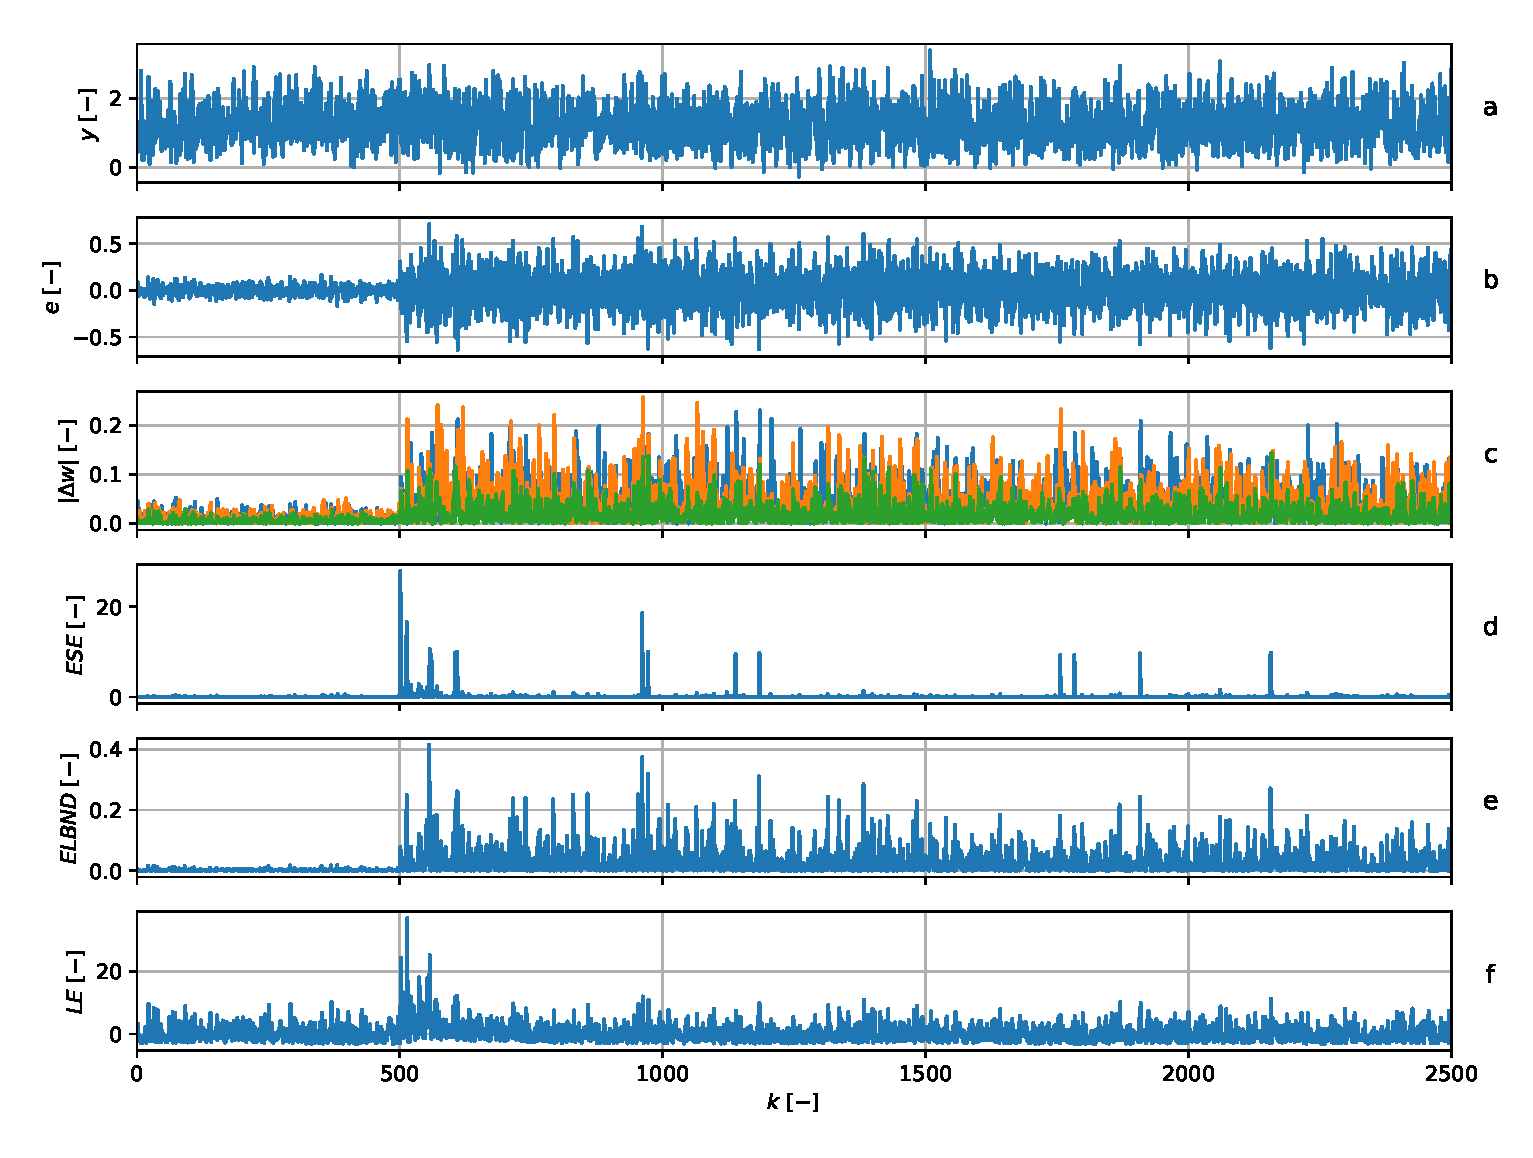
\includegraphics[scale=0.60]{IMG/mdpi/noise_change.eps}
    \caption{Detekce změny rozpylu šumu. Na grafu (a) jsou zobrazeny data z generátoru (modrá) a výstup z adaptivního filtru (zelená). Na grafu (b) je vynesena chyba filtru $e(k)$. Graf (c) zobrazuje velikosti přírůstků adaptivních parametrů filtru. Na grafu (d) jsou zobrazeny hodnoty ESE. V diskrétní časový okamžik $k=500$ je patrný značný nárůst v ESE, který reflektuje změnu směrodatné odchylky aditivního šumu. Na dalších grafech (e) a (f) jsou zobrazeny výsledné hodnoty algoritmů ELBND a LE.}
    \label{fig:noise_changed}
\end{figure}

\section{Detekce skokové změny parametrů generátoru signálu}\label{chap:mdpi_stepchange}
Tato případová studie je motivována problémem, který vzniká při sledování vícero náhodných datových toků \cite{stepchange} u kterých se kontroluje, zda nedošlo ke změně vlastností jejich generátoru. Uvažujme opět dva vstupy $x_1(k)$, $x_2(k)$ a výstup generátoru signálu ve tvaru
\begin{equation}
y(k)=x_1(k)+x_2(k)+x_1(k)\cdot x_2(k) + v(k)
\end{equation} 
kde člen $v(k)$ reprezentuje gaussovský aditivní šum s nulovou střední hodnotou a směrodatnou odchylkou $\sigma_n=0.1$, $v \sim N(0,0.1)$. Hodnoty vstupů $x_1(k)$ a $x_2(k)$ jsou v každém diskrétním časovém okamžiku náhodně vybrány z rovnoměrného rozdělení, $x_1(k) \sim U(0,1)$ resp. $x_2(k) \sim U(0,1)$. V časový diskrétní okamžik $k=500$ dojde ke změně parametrů generátoru, a výstup generátoru přejde do tvaru
\begin{equation}\label{eq:stepchange_dataset}
y(k)=0.4\cdot x_1(k) + 1.6x_2(k)+0.99x_1(k)\cdot x_2(k) + v(k).
\end{equation}
Jako adaptivní filtr byl v tomto případě zvolen QNU, jehož struktura odpovídá generátoru dat. Výstup tohoto filtru je tedy
\begin{equation}
\hat{y}(k)=w_1\cdot x_1(k)+w_2\cdot x_2(k)+w_3\cdot x_1(k)\cdot x_2(k)
\end{equation}
přičemž adaptivní parametry uvedeného filtru jsou adaptovány algoritmem GNGD.  Apriorní hodnota parametrů GPD a dat pro LE byla získána použitím 500 vzorků dat (vygenerovaných podle rovnice \ref{eq:stepchange_dataset}). Výsledky experimentu jsou znázorněny na obrázku \ref{fig:step_change}. Z obrázku je patrné, že pomocí algoritmu ESE se podařilo detekovat skokovou změnu parametrů, čemuž odpovídá výrazné globální maximum v ESE. Globální maximum v LE neodpovídá skokové změně parametrů generátoru a detekce pomocí algoritmu ELBND je opožděná.

\begin{figure}[h!]
    \centering
    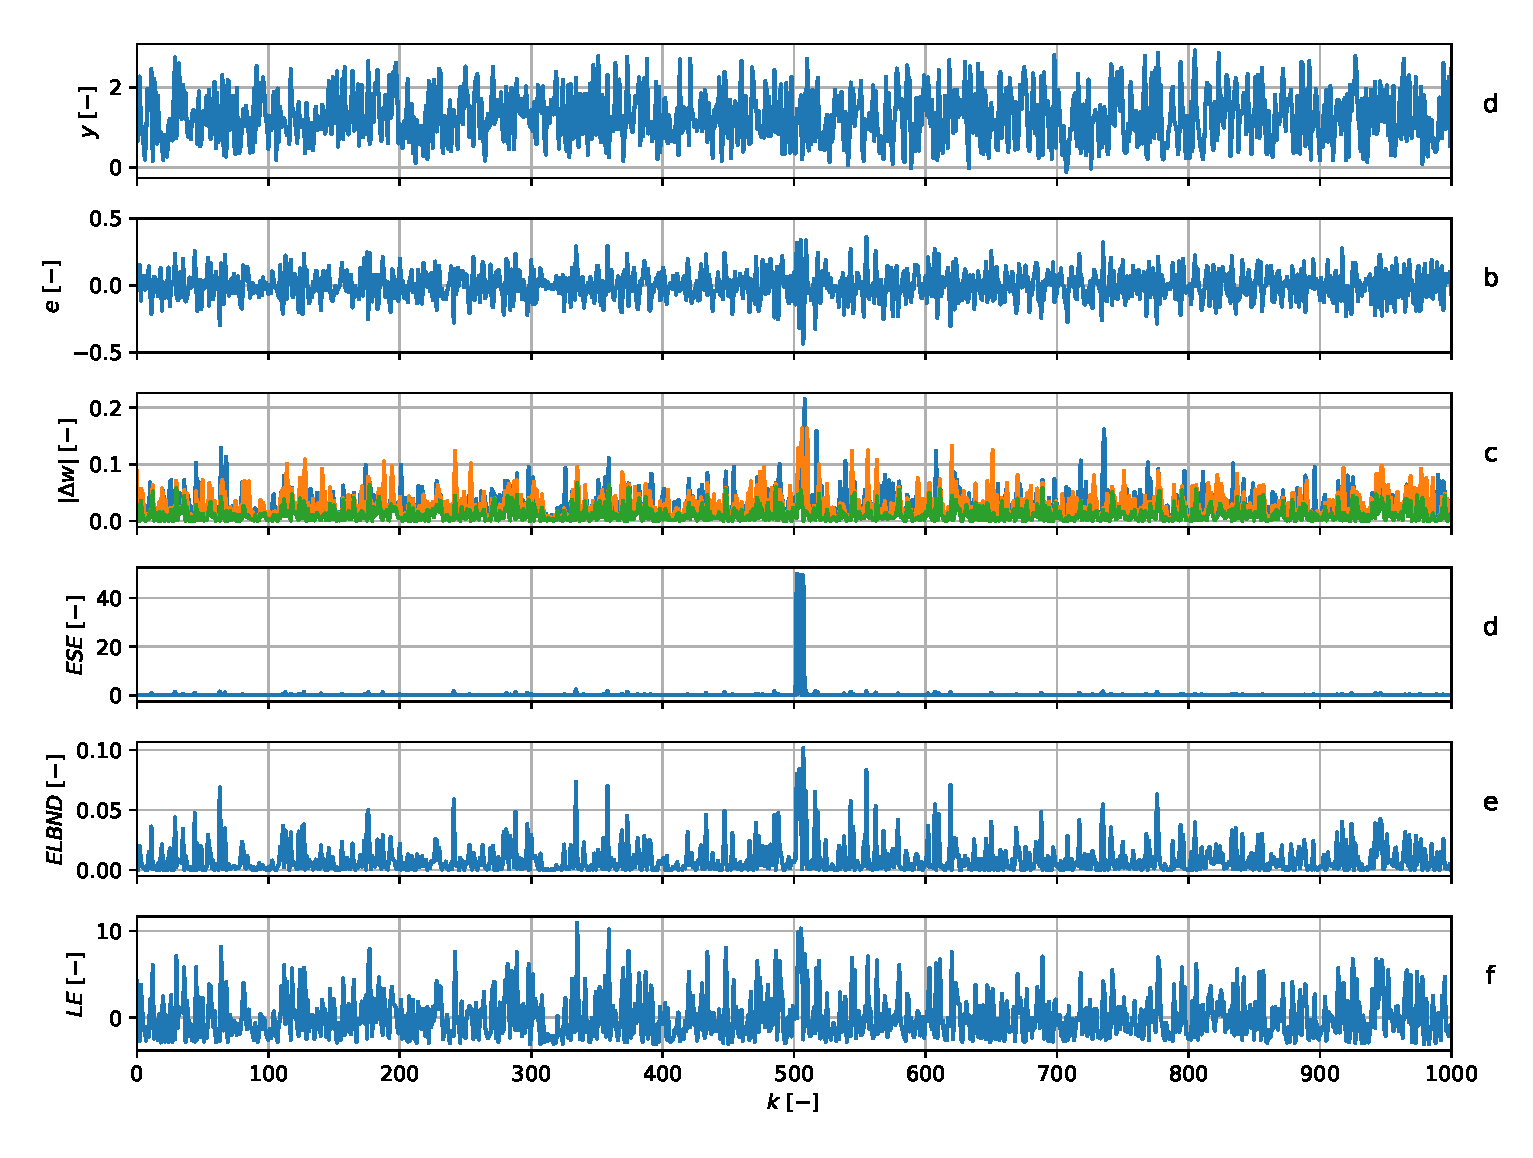
\includegraphics[scale=0.6]{IMG/mdpi/stepchange.eps}
    \caption{Detekce skokové změny generátoru signálu.Na grafu (a) je zobrazena původní časová řada (modrá). Graf (b) zobrazuje chybu filtru $e$. Na grafu (c) jsou zobrazeny velikosti přírůstků adaptivních vah filtru. Na grafu (d) jsou pak výsledky algoritmu ESE, přičemž k skokové změně parametrů generátoru signálu došlo v diskrétní časový okamžik $k=500$. Je tedy vidět globální maximum v ESE odpovídající úspěšné detekci. Na grafech (e) a (f) jsou pak výsledky metod ELBND a LE. Detekci algoritmem ELBND lze považovat za úspěšnou. Detekce algoritmem LE byla neúspěšná. Globální maximum LE je v diskrétním časovém okamžiku $k=338$, který neodpovídá skokové změně parametrů generátoru signálu.}
    \label{fig:step_change}
\end{figure}

\section{Detekce náhlé absence šumu}\label{chap:mdpi_noise_ext}
V této kapitole je ukázáno, že lehce modifikovaný algoritmus ESE může být využit také k detekci neobvykle malých změn parametrů adaptivního filtru. Oproti standardní variantě ESE budeme vyhodnocovat neobvykle malé přírůstky vah adaptivního filtru. Takže jediná změna v algoritmu je, že metodou POT budeme vybírat pouze nejmenší změny adaptivních vah a budeme odhadovat parametry GPD z takto vybraných hodnot.
\par
Uvažujme dva vstupy $x_1(k)$ a $x_2(k)$ jejichž hodnoty jsou v každém diskrétním časovém okamžiku $k$ vybrány z rovnoměrného rozdělení, takže  $x_1(k) \sim U(0,1)$ a $x_2(k)\sim U(0,1)$. Výstup generátoru dat $y(k)$ je definován jako
\begin{equation}
    y(k)=x_1(k)+x_2(k)+x_1(k)\cdot x_2(k)+v(k)
\end{equation}
kde člen $v(k)$ reprezentuje aditivní gaussovský šum s nulovou střední hodnotou a směrodatnou odchylkou $\sigma_n=0.1$. V diskrétním časovém okamžiku dojde k odstranění aditivního šumu a výstup generátoru signálu přejde do tvaru
\begin{equation}
    y(k)=x_1(k)+x_2(k)+x_1(k)\cdot x_2(k).
\end{equation}
který platí pro všechna $k\geq 500$.
\par 
Jako adaptivní filtr byl zvolen QNU, jehož výstup je definován
\begin{equation}
\hat{y}(k)=w_1\cdot x_1(k)+w_2\cdot x_2(k)+w_3\cdot x_1(k)\cdot x_2(k)
\end{equation}
takže jeho struktura odpovídá generátoru signálu. Parametry toho filtru jsou adaptovány algoritmem GNGD. Na obrázku \ref{fig:noise_ext} jsou zobrazeny výsledky experimentu. Maximum v ESE odpovídá detekci vymizení šumu z generátoru signálu. Výsledky metod ELBND a LE jsou uvedeny pouze pro ilustraci. 

\begin{figure}[ht!] 
    \centering
    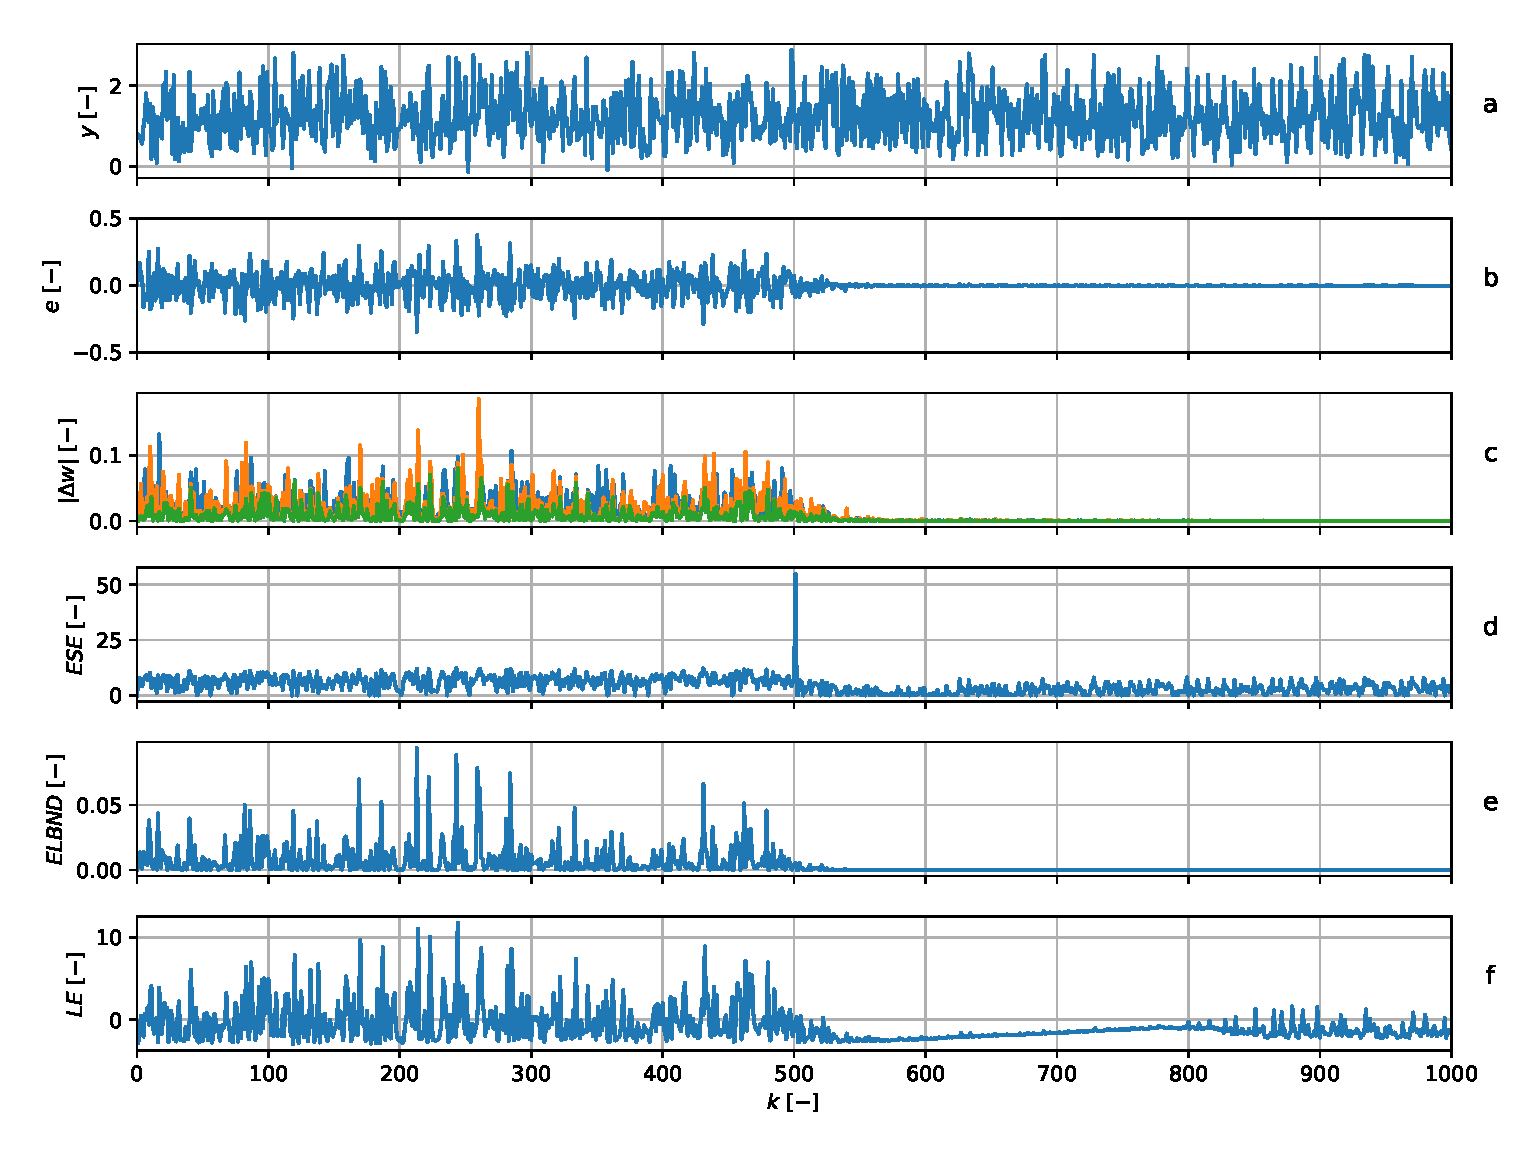
\includegraphics[scale=0.6]{IMG/mdpi/noise_ext.eps} 
    \caption{Detekce vymizení šumu ze signálu. Na grafu (a) je zobrazena původní časová řada (modrá). Graf (b) zobrazuje chybu filtru $e$. Na grafu (c) jsou zobrazeny velikosti přírůstků adaptivních vah filtru. Na grafu (d) jsou pak výsledky modifikovaného algoritmu ESE, přičemž k odstranění šumu ze signálu došlo v diskrétní časový okamžik $k=500$. Je tedy vidět globální maximum v ESE odpovídající úspěšné detekci vymizení šumu ze signálu. Na grafech (e) a (f) jsou pak výsledky získané pomocí metod ELBND a LE.}
    \label{fig:noise_ext}
\end{figure}

\section{Detekce změny trendu}\label{chap:mdpi_trendchange}
Cílem této kapitoly je demonstrovat použití algoritmu ESE při detekci změny trendu, což je úloha, která se často vyskytuje v oblasti detekce poruch a diagnostice \cite{diagnosis}. Uvažujme opět dva vstupy $x_1(k) \sim U(0,1)$ a $x_2(k)\sim U(0,1)$ a výstup generátoru dat $y(k)$ takový, že
\begin{equation}
    y(k)=x_1(k)+x_2(k)+0.01\cdot k + v(k)
\end{equation}
kde člen $v(k)$ reprezentuje aditivní gaussovský šum s nulovou střední hodnotou a směrodatnou odchylkou $\sigma_n=0.1$. V diskrétním časovém okamžiku $k=500$ nastane změna trendu. Výstup generátoru signálu se změní, tak, že
\begin{equation}
     y(k)=x_1(k)+x_2(k)+0.0105 \cdot k + v(k),
\end{equation}
pro $k\geq 500$. 
\par
Pro zpravování signálu byl použit filtr typu LNU s třemi vstupy, takže výstup uvedeného filtru je ve tvaru
\begin{equation}
    \hat{y}(k)=w_1\cdot x_1(k)+w_2\cdot x_2(k)+w_3
\end{equation}
takže odpovídající vektor vstupů je
\begin{equation}
    \textbf{x}(k)=[x_1(k),x_2(k),1].
\end{equation}
Struktura LNU byla vybrána tak, aby co nejlépe odpovídala struktuře generátoru signálu. Parametry adaptivního filtru byly v tomto experimentu adaptovány algoritmem GNGD. Na obrázku \ref{fig:trend_change} jsou zobrazeny výsledky experimentu. Globální maximum ESE odpovídá okamžiku změny trendu. Algoritmy LE a ELBND úspěšně změnu trendu také detekovali.
\begin{figure}[ht!]

    \centering
    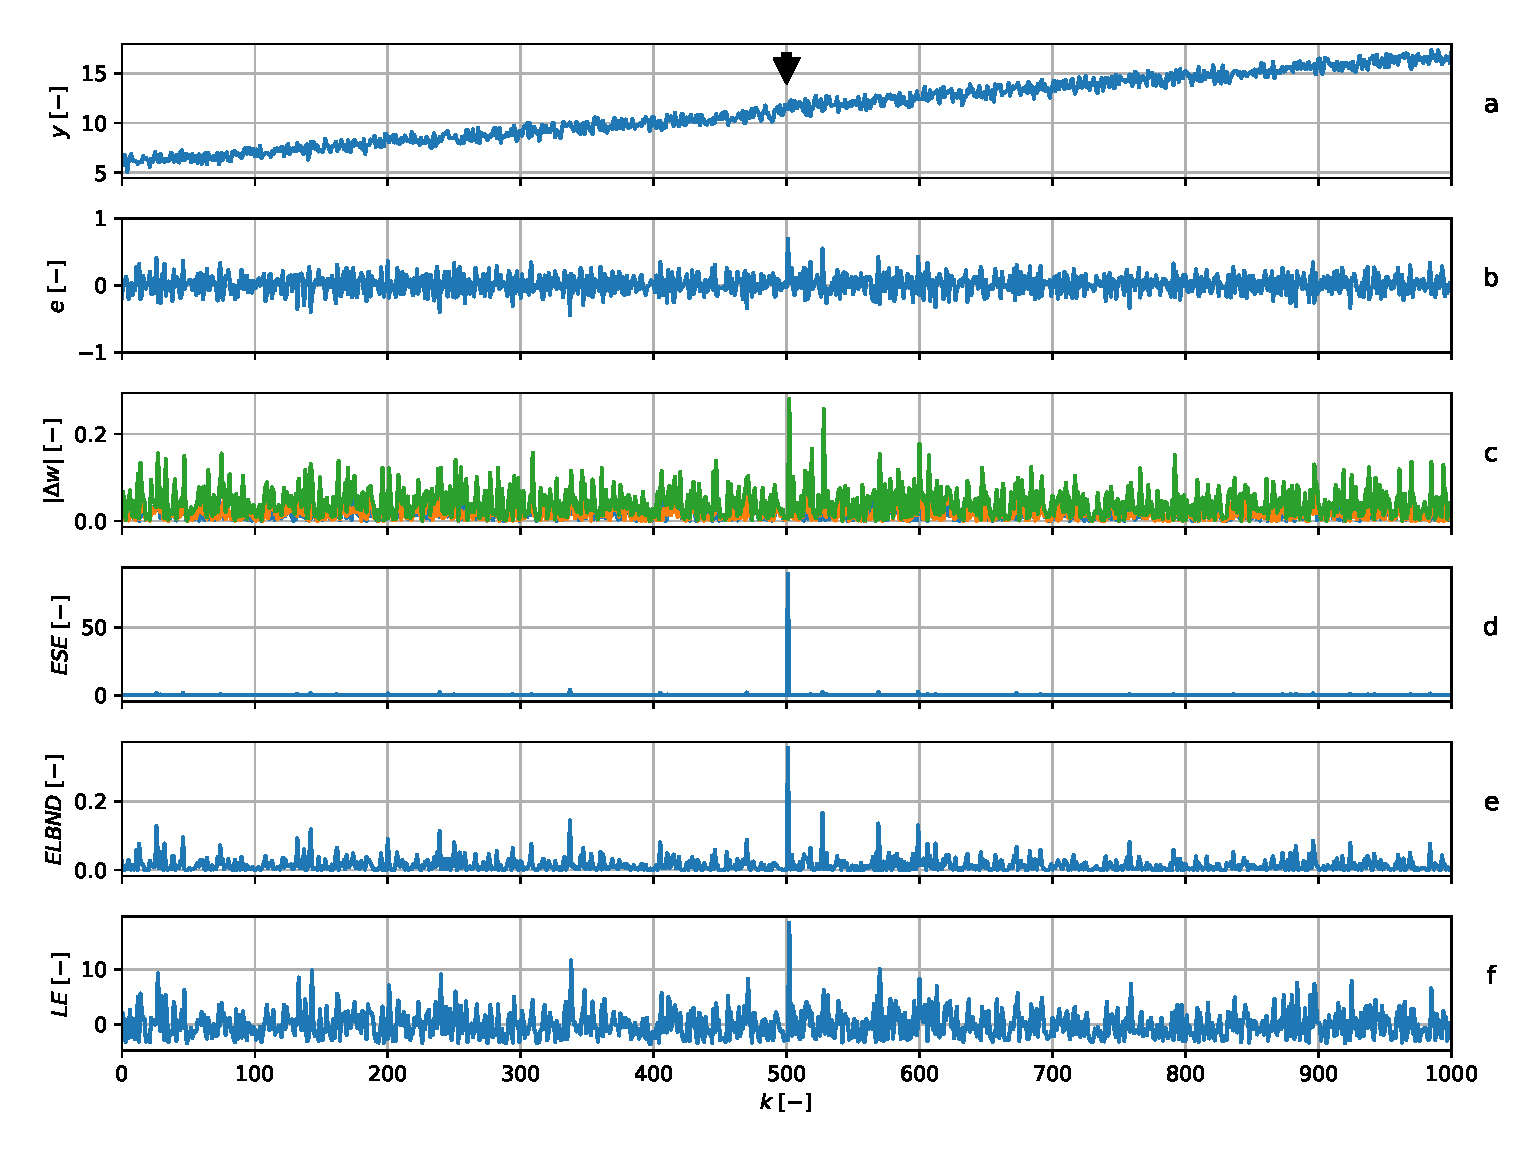
\includegraphics[scale=0.60]{IMG/mdpi/trendchange.eps}
    \caption{Detekce změny trendu při použití algoritmu GNGD. Na grafu (a) jsou zobrazena data z generátoru signálu (modré). Černá šipka znázorňuje okamžik ve kterém došlo ke změně trendu. Na grafu (b) je zobrazena chyba adaptivního filtru $e$. Na grafu (c) jsou znázorněny velikosti přírůstků adaptivních vah filtru. Grafy (d), (e) a (f) znázorňují výsledky detekce novosti pomocí algoritmů ESE, ELBND a LE. Všechny tři algoritmy vykazují úspěšnou detekci změny trendu, která koresponduje s jejich maximální hodnoty během experimentu.}
\label{fig:trend_change}
\end{figure}
\par

\section{Detekce epilepsie v EEG záznamu myši}\label{chap:mdpi_eeg}
Poslední případová studie je věnována detekci epileptického záchvatu v signálu EEG myši pomocí algoritmu EEG. Standartizovaná data ze tří vybraných kanálů EEG, ve kterých byl expertem stanoven začátek epileptického záchvatu přibližně v čase $k \approx 1700$, jsou zobrazeny na obrázku \ref{fig:eeg_seizure}. Standartizace byla provedena podle předpisu
\begin{equation}
y=\frac{x-\mu_{x}}{\sigma_{x}}
\end{equation}
kde $y$ je výsledná standartizovaná hodnota, $x$ je původní hodnota, $\mu_x$ je průměrná hodnota původních dat daného kanálu a $\sigma_x$ je jejich původní směrodatná odchylka.
\par
Jako adaptivní filtr byl, na základě experimentů, zvolen FIR filtr délky 10. Vstupem je vektor dat
\begin{equation}
\textbf{x}=[x(k-1_,x(k-2),\dots,x(k-10)]
\end{equation}
takže filtr má 10 adaptivních parametrů. Filtr byl adaptován algoritmem NLMS.  Výsledky detekce algoritmem ESE jsou zobrazeny na obrázku \ref{fig:mouse_novelty}. Pozice globálního maxima ESE v kanálu C3 (obzvláště signifikantní) je v diskrétním časovém okamžiku $k=1735$, v kanálu Pz je to  $k=1698$ a v kanálu Fp1 je to v $k=1727$. 

\begin{figure}[ht!]
    \centering
    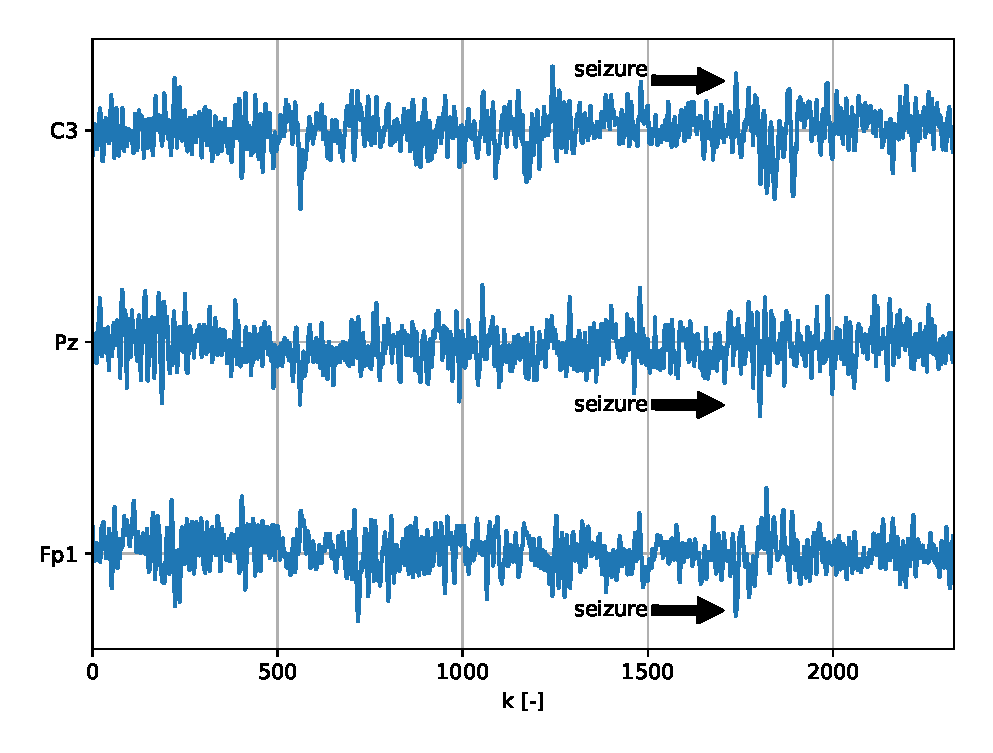
\includegraphics[scale=0.88]{IMG/mdpi/mouse_eeg.eps}
    \caption{Vybrané kanály myšího EEG na kterých je patrný epileptický záchvat. Data byly standartizovány. Začátek záchvatu je přibližně v $k\approx 1700$, což znázorňuje černá šipka.}
    \label{fig:eeg_seizure}
\end{figure}
\begin{figure}[ht!]
    \centering
    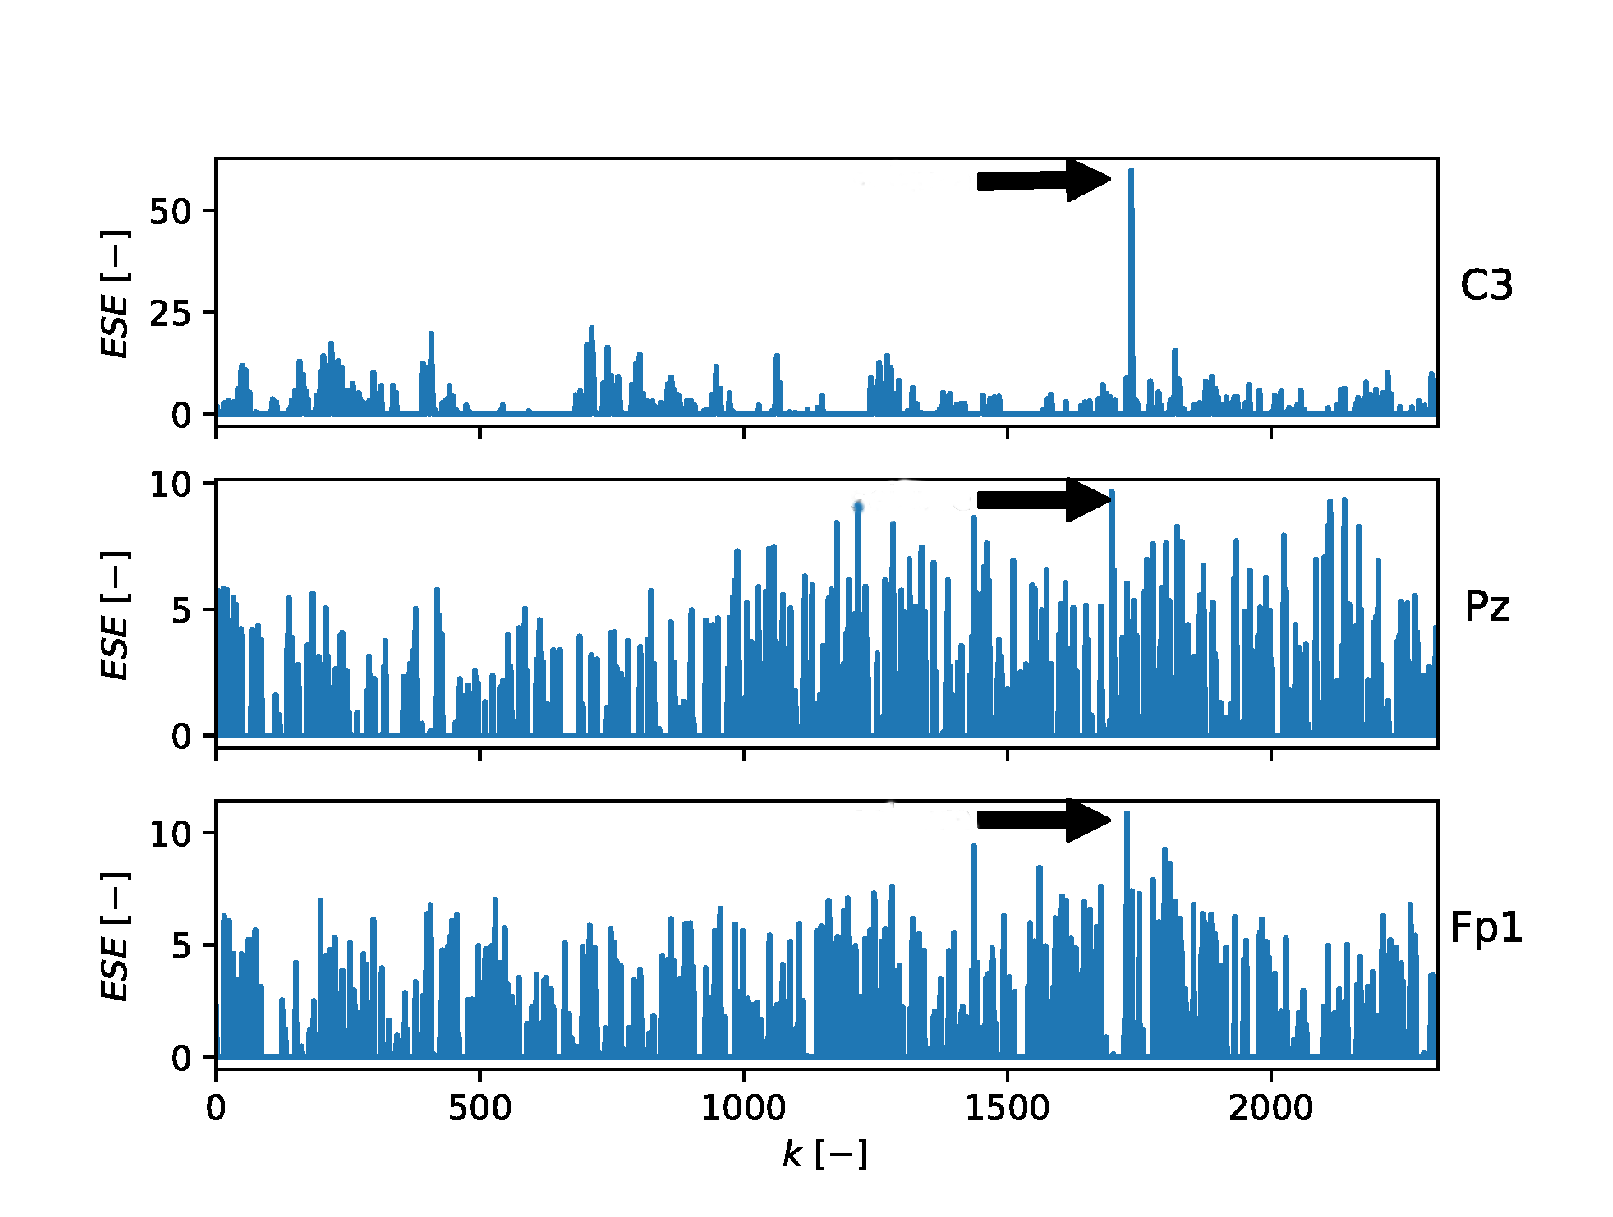
\includegraphics[scale=0.58]{IMG/mdpi/mouse_novelty.eps}
    \caption{Hodnota ESE pro vybrané kanály se záznamem myšího EEG ve kterých je patrný epileptický záchvat. V kanále C3 je v ESE výrazný nárůst po začátku záchvatu (přibližně v $k \approx 1700$), v porovnání s ostatními kanály. Černá šipka znázorňuje přibližný začátek epileptického záchvatu.}
    \label{fig:mouse_novelty}
\end{figure}


\section{Vyhodnocení úspěšnosti detekce skokové změny parametrů generátoru signálu}\label{chap:mdpi_step_stats}
Pro vyhodnocení úspěšnosti skokové změny parametrů generátoru signálu uvažujme generátor signálu s dvěma vstupy $x_1(k)$ a $x_2(k)$ a výstupem $y(k)$ ve tvaru
\begin{equation}
y(k)=a_1\cdot x_1(k)+a_2\cdot x_2(k)+a_3\cdot x_1(k) \cdot x_2(k)+v(k)
\end{equation}
kde člen $v(k)$ reprezentuje gaussovský aditivní šum s nulovou střední hodnotou a směrodatnou odchylkou $\sigma$. Počáteční hodnoty parametrů $a_1$, $a_2$ a $a_3$ jsou vygenerovány z rovnoměrného rozdělení $U(-1,1)$. V diskrétním časovém okamžiku $k=200$, dojde ke skokové změně těchto parametrů a jejich nová hodnota je opět náhodně vygenerována z rovnoměrného rozdělení $U(-1,1)$. Celkový počet vzorků experimentu je 400.
Použitý adaptivní filtr je stejný jako v předchozí případové studii detekce skokové změny parametrů generátoru signálu, viz kapitola \ref{chap:mdpi_stepchange}. Parametry tohoto adaptivního filtru byly adaptovány algoritmem GNGD. Apriorní informace o parametrech GPD byla pro každý experiment získána pomoci 1200 vzorků, s počátečními hodnotami parametrů $a_1$, $a_2$ a $a_3$. Pro každý experiment byla vyhodnocena hodnota SNR jako
\begin{equation}\label{eq:snr}
SNR=10\log_{10}\frac{\sigma_s^2}{\sigma_n^2}
\end{equation}
kde $\sigma_s$  je hodnota směrodatné odchylky výstupu generátoru signálu během experimentu a $\sigma_n$ je směrodatná odchylka aditivního gaussovského šumu. Vyhodnocení přesnosti detekce bylo provedeno následujícím způsobem:
\begin{enumerate}
\item nastavení hodnoty směrodatné odchylky šumu $\sigma_n$
\item pro zvolenou hodnotu směrodatné odchylky $\sigma_n$ se provede 1000 experimentů, přičemž pro každý experiment jsou nově vygenerovány počáteční hodnoty parametrů generátoru signálu $a_1$, $a_2$ a $a_3$.
\item pro každý experiment je vyhodnocena úspěšnost detekce. Za úspěšnou detekci je považováno, pokud globální maximum ESE, ELBND, EL respektive chyby filtru je v mezích $k\geq 200$ a $k\leq 210$. 
\item vypočte se celková úspěšnost detekce pro danou hodnotu směrodatné odchylky (poměr počtu úspěšných detekcí k celkovému počtu experimentů)
\item pro každý experiment se vyhodnotí SNR podle \ref{eq:snr} a pak se pro zvolenou hodnotu $\sigma$ vypočítá průměrná hodnota $SNR$ pro všechny experimenty
\end{enumerate}
Vyhodnocení úspěšnosti detekce bylo vyhodnoceno pro dva případy. V prvním případě, byly hodnoty vstupů $x_1(k)$ a $x_2(k)$ generovány z rovnoměrného rozdělení $U(-1,1)$. Výsledky úspěšnosti detekce pro různé hodnoty směrodatných odchylek šumu $\sigma_n$ jsou zobrazeny na obrázku \ref{fig:step_uni_stats}. Pro porovnání jsou zvoleny metody ELBND , LE s oknem $n_s=1200$ a velikost chyby adaptivního filtru $e$ (v grafu označeno jako ERR).

\begin{figure}[!ht]
    \centering
    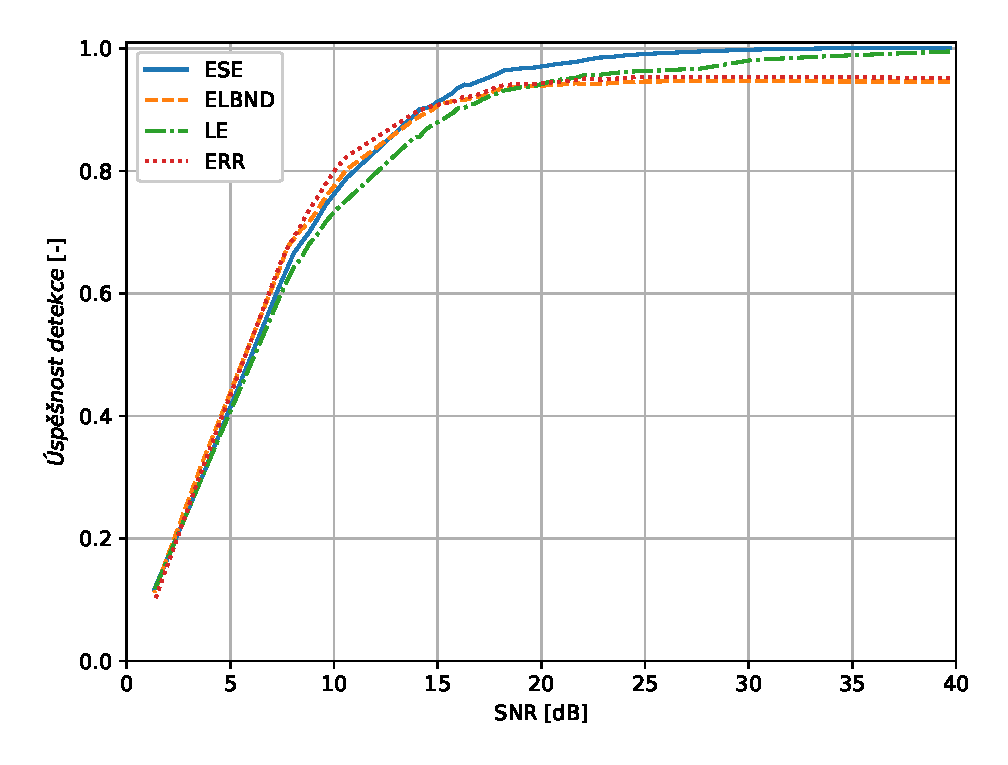
\includegraphics[scale=0.66]{IMG/mdpi/stepuni_stats.eps}
    \caption{Úspěšnost detekce skokové změny parametrů generátoru signálu. Hodnoty vstupů generátoru signálu jsou generovány z rovnoměrného rozdělení $U(-1,1)$. 
Pro hodnoty $SNR > 15$ $dB$ dosáhl algoritmus ESE vyšší úspěšnost než algoritmy  LE, ELBND a vyhodnocení pomocí chyby filtru (ERR). Pro $SNR > 33$ $dB$ dosáhl algoritmus ESE 100\% úspěšnost detekce.}
    \label{fig:step_uni_stats}
\end{figure}
Ve druhém případě byly hodnoty vstupů $x_1(k)$ a $x_2(k)$ generovány z normálního rozdělení. Vyhodnocení úspěšnosti detekce bylo provedeno stejně jako v případě popsaném výše. Výsledky úspěšnosti detekce pro různé hodnoty směrodatných odchylek šumu $\sigma_n$ jsou zobrazeny na obrázku \ref{fig:step_norm_stats}.

\begin{figure}[!h]
    \centering
    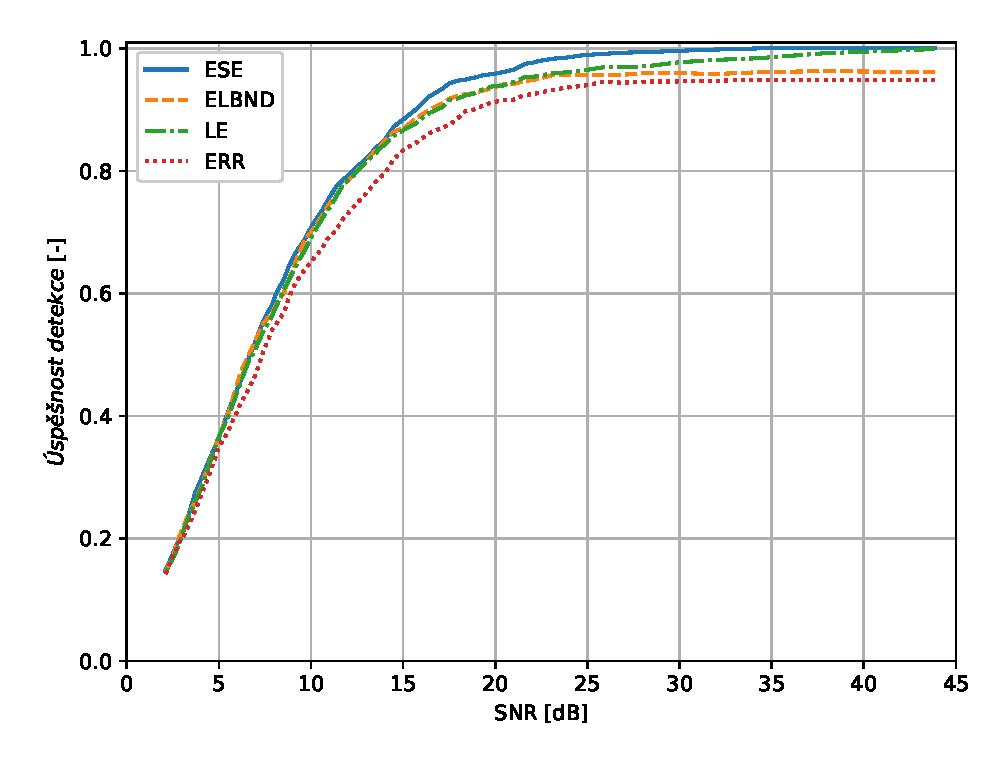
\includegraphics[scale=0.66]{IMG/mdpi/stepnorm_stats.eps}
    \caption{Úspěšnost detekce skokové změny parametrů signálu. Hodnoty vstupů generátoru signálu jsou generovány z normálního rozdělení $N(0,1)$. Pro hodnoty $SNR > 8$ $dB$ dosáhl algoritmus ESE  lepší úspěšnosti detekce než algoritmy LE, ELBND a vyhodnocení pomocí velikosti chyby predikce (ERR). Pro $SNR > 34$ $dB$ dosáhl algoritmus ESE 100\% úspěšnosti detekce.}
    \label{fig:step_norm_stats}
\end{figure}


\section{Vyhodnocení úspěšnosti detekce skokové změny trendu}\label{chap:mdpi_trendchange_evaluation}
Pro vyhodnocení úspěšnosti změny trendu uvažujme výstup generátoru signálu $y(k)$ se dvěma vstupy $x_1(k)$ a $x_2(k)$ jehož výstup je definován jako
\begin{equation}\label{eq:trnd_stats}
    y(k) = x_1(k) + x_2(k) + 0.01 \cdot k + v(k)
\end{equation}
kde člen $v(k)$ reprezentuje aditivní gaussovký šum s nulovou střední hodnotou a směrodatnou odchylkou $\sigma_n$. V diskrétním časovém okamžiku $k=200$ se změní výstup generátoru signálu
\begin{equation}
    y(k) = x_1(k) + x_2(k) + (0.01 + a) \cdot k + v(k)
\end{equation}
přičemž parametr $a$ je vygenerován v každém experimentu z rovnoměrného rozdělení $U(-0.02,0.02)$. Počet vzorků experimentu je 400.
\par 
Struktura adaptivního filtru byla zvolena stejně jako v předcházející případové studii detekce změny trendu (viz kapitola \ref{chap:mdpi_stepchange}). Adaptivní parametry filtru byly adaptovány algoritmem GNGD. Apriorní informace o parametrech GPD byla získána na základě 1200 vzorků, ve kterých nedošlo ke změně trendu. 
\par 
Vyhodnocení přesnosti detekce změny trendu bylo provedeno následujícím způsobem:
\begin{enumerate}
\item nastavení hodnoty směrodatné odchylky šumu $\sigma_n$
\item pro zvolenou hodnotu směrodatné odchylky $\sigma_n$ se provede 1000 experimentů. V každém experimentu dojde v diskrétním časovém okamžiku $k=200$ k  novému vygenerování hodnoty parametru $a$ z rovnoměrného rozdělení $U(-0.02,0.02)$.
\item pro každý experiment je vyhodnocena úspěšnost detekce. Za úspěšnou detekci je považováno, pokud globální maximum ESE, ELBND, EL respektive chyby filtru je v mezích $k\geq 200$ a $k\leq 210$. 
\item vypočte se celková úspěšnost detekce pro danou hodnotu směrodatné odchylky šumu $\sigma_n$ (poměr počtu úspěšných detekcí k celkovému počtu experimentů)
\item pro každý experiment se vyhodnotí SNR podle \ref{eq:snr} a pak se pro zvolenou hodnotu $\sigma_n$ vypočítá průměrná hodnota $SNR$ pro všechny experimenty
\end{enumerate}

Vyhodnocení úspěšnosti detekce změny trendu bylo vyhodnoceno pro hodnoty vstupů $x_1(k)$ a $x_2(k)$ vygenerovány z rovnoměrného rozdělení $U(-1,1)$. Výsledky úspěšnosti detekce pro různé hodnoty směrodatných odchylek šumu $\sigma_n$ jsou zobrazeny na obrázku \ref{fig:trend_stats}. Pro porovnání jsou zvoleny metody ELBND, LE s oknem $n_s=1200$ (výpočet podle rovnice a velikost chyby adaptivního filtru $e$ (v grafu označeno jako ERR).

\begin{figure}[!ht]
    \centering
    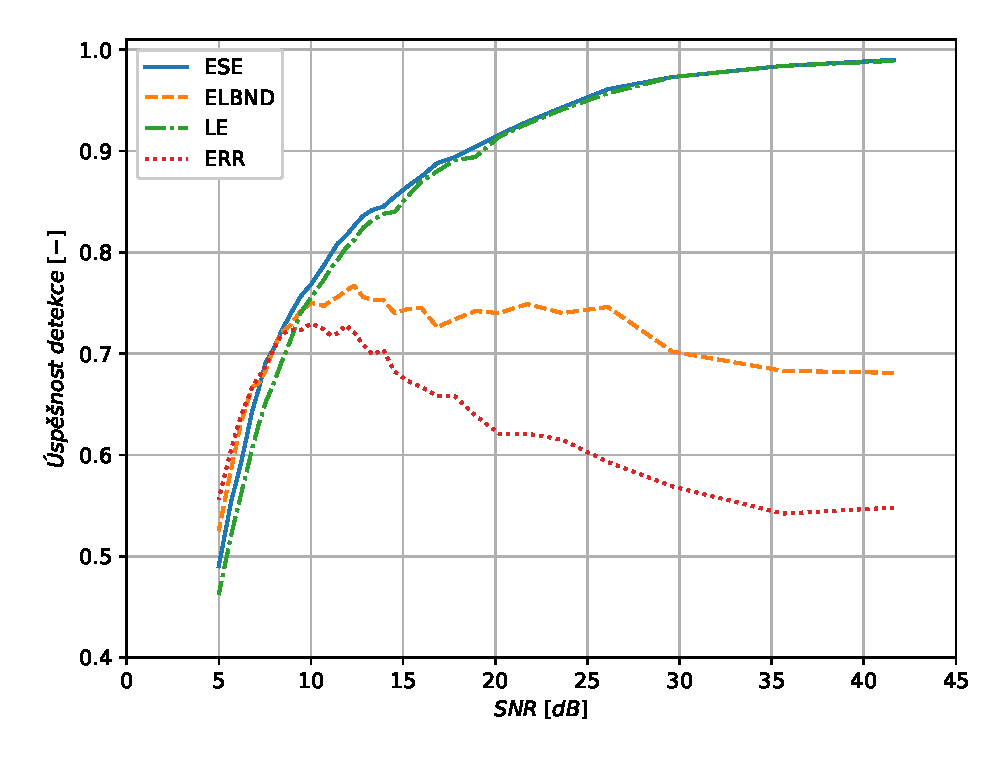
\includegraphics[scale=0.66]{IMG/mdpi/trendchange_stats.eps}
    \caption{Úspěšnost detekce změny trendu. Hodnoty vstupů generátoru signálu byly generovány z rovnoměrného rozdělení $U(-1,1)$. Pro hodnoty $SNR > 8$ $dB$ dosáhl algoritmus ESE větší úspěšnosti detekce než LE, ELBND a vyhodnocení pomocí velikosti chyby filtru.}
    \label{fig:trend_stats}
\end{figure}


\section{Evaluace ROC křivky pro detekci změny trendu}\label{chap:appel_roc}
Protože úspěšná detekce novosti pomocí algoritmu ESE je závislá na volbě hodnoty, od které budeme považovat hodnotu ESE za \textquote{novost}, byl proveden experiment detekce změny trendu a vyhodnocena ROC (Receiver Operating Characteristics) křivka \cite{roc_orig}. ROC křivka poskytuje vhodný způsob jak vizualizovat schopnost binárního klasifikátoru klasifikovat správně data na základě proměnlivé velikosti prahu, který klasifikaci určuje (v případě algoritmu ESE je to hodnota ESE) a zároveň umožňuje objektivně jednotlivé klasifikátory porovnávat \cite{roc_bible} (více viz následující podkapitola \ref{chap:roc_specs}). Pro porovnání algoritmu ESE byly opět zvoleny algoritmy LE, ELBND a klasifikátor, který klasifikuje vzorky náhodně.
\par Výsledky uvedené v této kapitole byli publikovány v \ref{appel3}.
\subsection{Popis experimentu}
Stejně jako v případě vyhodnocení přesnosti detekce změny trendu (viz podkapitola \ref{chap:mdpi_trendchange_evaluation}) i v tomto experimentu uvažujeme dva vstupy $x_1(k)$ a $x_2(k)$ výstup generátoru signálu $y(k)$ ve tvaru 
\begin{equation}
    \label{eq:trend}
    d(k)=x_1(k)+x_2(x)+0.01\cdot k + v(k)
\end{equation}
\begin{equation*}
0\leq k < 200
\end{equation*}
kde člen $v(k)$ reprezentuje gaussovský aditivní šum s nulovou střední hodnotou a směrodatnou odchylkou $\sigma_n$. V diskrétním časovém okamžiku $k=200$ přejde výstup generátoru signálu do tvaru
\begin{equation}
y(k)=x_1(k)+x_2(x)+(0.01 + a)\cdot k + v(k)
\end{equation}
\begin{equation*}
200 \leq k \leq 399
\end{equation*}
přičemž hodnota parametru $a$ je vygenerována z rovnoměrného rozdělení $U(-0.02,0.02)$ a pro všechna $200 \leq k \leq 399$ je během daného experimentu konstantní. Hodnoty vstupů $x_1(k)$ a $x_2(k)$ jsou generovány z rovnoměrného rozdělení $U(-1,1)$. 
\par 
Jako adaptivní filtr byl zvolen QNU, jehož struktura odpovídá struktuře generátoru signálu. Výstup adaptivního filtru je ve tvaru
\begin{equation}
\hat{y}(k)=w_1\cdot x_1(k)+w_2\cdot x_2(k) + w_3 \cdot x_1(k) \cdot x_2(k)
\end{equation}
a parametry toho adaptivního filtru byly adaptovány algoritmem GNGD.
\par 
Apriorní hodnota parametrů GPD pro algoritmus ESE je získána pomocí 1200 vzorků, získaných z výstupu generátoru signálu, který je dán rovnicí \ref{eq:trend}. Během experimentů byla délka okna $n_s=1200$. Výsledky algoritmu LE byly získány pro okno délky $M=1200$. Pro každou hodnotu $\sigma$ bylo provedeno 10000 experimentů na jejichž základě byla zkonstruována ROC křivka. Hodnoty směrodatných odchylek $\sigma_n$ byly vybrány takto:
\begin{equation}
\sigma_n=\{0.1,0.2,0.5,1.0,2.0,2.5 \}
\end{equation}
a pro každou hodnotu $\sigma_n$ byla pro všech 10000 experimentů určená průměrná hodnota $SNR$, která byla pro každý experiment vypočtena podle rovnice $\ref{eq:snr}$. 

\subsection{Konstrukce ROC křivky}\label{chap:roc_specs}
Pro konstrukci ROC křivky je důležité, aby množina výsledků byla vyvážená. Tedy aby obsahovala stejný počet pozitivních i negativních vzorků. Pro získání vyvážené množiny výsledků byl nejdřív každý experiment převzorkován podle následujícího předpisu
\begin{equation}
    ND_r(i) = max\{ND(i \cdot 10), ND(i \cdot 10 + 1), ND(i \cdot 10 + 2), \dots, ND(i \cdot 10 + 9)\}
\end{equation}
\begin{equation*}
i = 0,1,\dots,39
\end{equation*}
kde $ND$ reprezentuje hodnotu detektoru novosti (resp. hodnoty algoritmu ESE, ELBND, LE). Z každé převzorkované datové řady jsou vygenerovány dvě množiny. Množina $P$ obsahuje pozitivní vzorek, takový, že $P=\{ND_r(20)\}$ (protože v diskrétním časovém okamžiku $k=200$ došlo ke změně trendu).  Množina $N$ obsahuje obsahuje zbylých 39 negativních vzorků, takže $N=\{ND(0), \dots ND(19), ND(21), \dots ND(39) \}$. Při konstrukci ROC křivky jsou pro každý experiment vybrány dva vzorky. Jeden vzorek z množiny $P$ a jeden náhodně vybraný vzorek z množiny $N$. Pro vyhodnocení ROC je klíčové zjistit, jestli jsou pozitivní vzorky (prvky množiny $P$) pro daný práh správně klasifikovány jako pozitivní (True Positive) a zda-li jsou negativní vzorky klasifikovány jako falešně pozitivní (False Positive). Pro danou velikost prahu se určí úspěšnost detekce skutečně pozitivních (True Positive Rate) jako 
\begin{equation}
TPR=\frac{TP}{P}=\frac{TP}{10000}
\end{equation}
kde $TP$ je počet správně pozitivně klasifikovaných vzorků a $P$ je celkový počet skutečně pozitivních vzorků. Dále je potřeba určit poměr falešně pozitivních (False Positive Rate) vzorků pro daný práh jako
\begin{equation}
FPR=\frac{FP}{N}=\frac{FP}{10000}
\end{equation}
kde $FP$ je počet vzorků klasifikovaných jako falešně pozitivní a $N$ je celkový počet skutečně negativních vzorků. ROC pak zobrazuje závislost úspěšnost detekce skutečně pozitivních vzorků ($TPR$) v závislosti na poměru falešně pozitivních vzorků ($FPR$).
\par 
Hodnota $TPR$ bývá nazývána také jako sensitivita. Komplementární hodnotou k $FPR$ je potom specifita (True Negative Rate $TNR$), která určuje, kolik opravdu negativních vzorku ($TN$) je klasifikováno jako negativní. Komplementární ve smyslu
\begin{equation}
TNR=\frac{TN}{N}=1-FPR.
\end{equation} 
Komplementární k sensitivitě je hodnota míry falešně negativních ($FNR$), která určuje poměr falešně negativních k ($FN$) k celkovému počtu pozitivních, tedy
\begin{equation}
FNR=\frac{FN}{P}=1-TPR.
\end{equation}
\par 
Pro každou ROC křivku je možné určit plochu pod touto křivkou AUROC (Area Under ROC), která vypovídá o schopnosti klasifikátoru rozlišovat mezi jednotlivými třídami. Čím větší plocha pod křivkou, tím víc klasifikátor správně klasifikuje pozitivní případy jako pozitivní a negativní případy jako negativní. Plocha AUROC ideálního klasifikátoru bude 1, zatímco plocha nejhoršího možného klasifikátoru bude rovna 0 (tento klasifikátor, ale bude dokonalým klasifikátorem, pokud zaměníme označení negativní třídy za pozitivní). Plocha AUROC náhodného klasifikátoru bude 0.5, neboť tento klasifikátor nedokáže vůbec rozlišovat mezi pozitivními a negativními případy.
\subsection{Výsledky experimentu}
Výsledné ROC křivky pro různé hodnoty $SNR$ jsou zobrazeny v obrázcích \ref{fig:roc_01}-\ref{fig:roc_25}. Modrá čára zobrazuje výsledky algoritmu ESE, zelená tečkovaná čára zobrazuje výsledky algoritmu LE, červená přerušovaná čára výsledky algoritmu ELBND a černá čerchovaná čára zobrazuje výsledky náhodného klasifikátoru. 
\par 
Pro každou ROC křivku byla vypočtena hodnota plochy pod touto křivkou, AUROC, pomocí lichoběžníkové metody, jako
\begin{equation}
AUROC \approx \sum_{j=1}^{n_t} \frac{TPR(FPR(j))+TPR(FPR(j+1))}{2} \cdot(FPR(j+1)-FPR(j))
\end{equation}
kde $n_t$ reprezentuje počet vyhodnocovaných prahů zmenšený o 1. Výsledné plochy pod křivkami ROC jsou pro jednotlivé metody a směrodatné odchylky šumu uvedené v následující tabulce \ref{tab:auroc}. Tučně je zvýrazněna nejvetší hodnota AUROC. Podle uvedených hodnot při průměrném $SNR=35.8$ nejlépe rozlišuje mezi pozitivními a negativními případy algoritmus LE. Pro nižší hodnoty $SNR$ je nejlépe separujícím algoritmem ESE.
\begin{table}[h!]

\caption{$AUROC$ pro detekci změny trendu}
\centering
\begin{tabular}{|l|c|c|c|c|}
\hline
\multicolumn{2}{|l|}{} & \multicolumn{3}{c|}{\textbf{AUROC}} \\ \hline
$\sigma_n$ & \textit{SNR [dB]} & \textit{ESE} & \textit{LE} & \textit{ELBND} \\ \hline
0.1 & 35.8 & 0.9954 & \textbf{0.9952} & 0.8234\\ \hline
0.2 & 30.0 & \textbf{0.9920} & 0.9912 & 0.8299 \\ \hline
0.5 & 21.7 & \textbf{0.9816} & 0.9777 & 0.8288 \\ \hline
1.0 & 16.2 & \textbf{0.9576} & 0.9496 & 0.8263 \\ \hline
2.0 & 10.8 & \textbf{0.9286} & 0.9214 & 0.8397 \\ \hline
2.5 & 9.2 & \textbf{0.9134} & 0.9056 & 0.8446 \\ \hline
\end{tabular}
\label{tab:auroc}
\end{table}
V další tabulce \ref{tab:dr} je uvedená úspěšnost klasifikace, kde za úspěšnou klasifikaci je považován případ, kdy maximální hodnota ESE, ELBND nebo LE během experimentu je v intervalu $200\leq k\leq210$, tedy do deseti vzorků po změně trendu.
\begin{table}[h!]
\caption{Úspěšnost detekce změny trendu}
\centering
\begin{tabular}{|l|c|c|c|c|}
\hline
\multicolumn{2}{|l|}{} & \multicolumn{3}{c|}{\textbf{Úspěšnost detekce}} \\ \hline
$\sigma_n$ & \textit{SNR [dB]} & \textit{ESE} & \textit{LE} & \textit{ELBND} \\ \hline
0.1 & 35.8 & 98.88 & \textbf{98.92} & 60.00 \\ \hline
0.2 & 30.0 & \textbf{98.14} & 98.03 & 59.61 \\ \hline
0.5 & 21.7 & \textbf{95.18} & 95.08 & 59.65 \\ \hline
1.0 & 16.2 & \textbf{90.42} & 89.96 & 57.67 \\ \hline
2.0 & 10.8 & \textbf{81.27} & 78.51 & 57.69 \\ \hline
2.5 & 9.2 & \textbf{75.86} & 71.56 & 57.16 \\ \hline
\end{tabular}
\label{tab:dr}
\end{table}
Tučně jsou zvýrazněny hodnoty nejvyšší úspěšnosti detekce. Z výsledků je patrné, že pro průměrné $SNR=35.8$ má nejvyšší úspěšnost algoritmus LE. Pro nižší hodnoty $SNR$ je algoritmem s nejvyšší úspěšností detekce algoritmus ESE.
\begin{figure}[ht!]
    \centering
    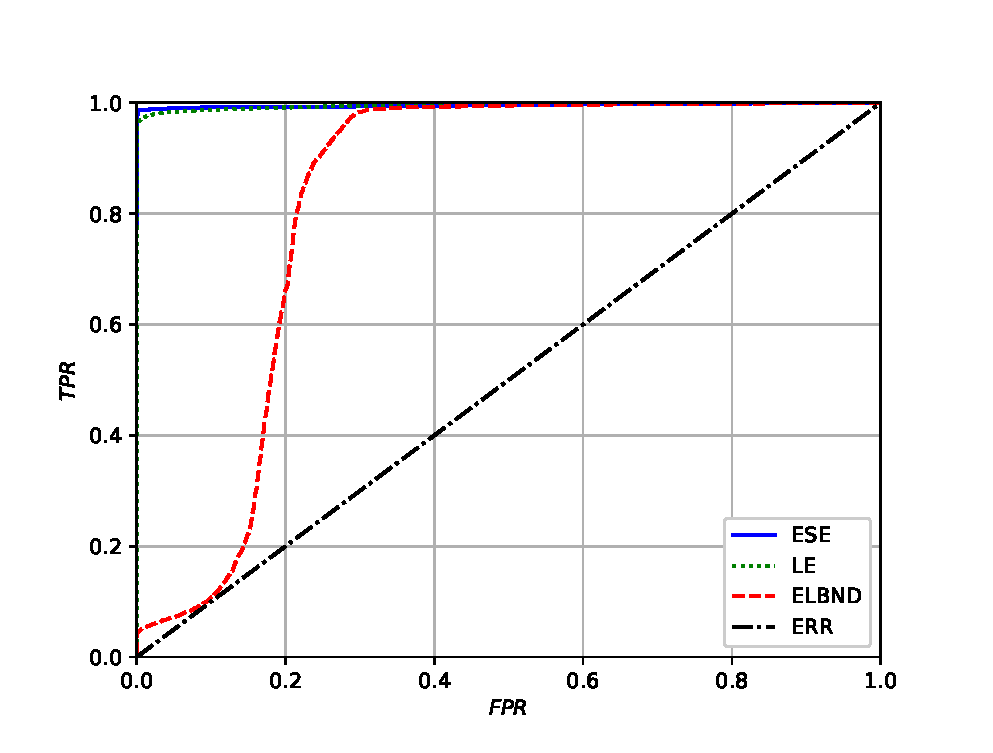
\includegraphics[scale=0.7]{IMG/appel_roc/roc_01.eps}
    \caption{ROC křivky v případě detekce změny trendu signálu obsahujícího aditivní gaussovský šum se směrodatnou odchylkou $\sigma=0.1$. Průměrná hodnota $SNR$ experimentů byla $SNR=35.80$ $dB$. Černá čerchovaná čára (RANDOM) reprezentuje náhodný klasifikátor.}
    \label{fig:roc_01}
\end{figure}
\begin{figure}[ht!]
    \centering
    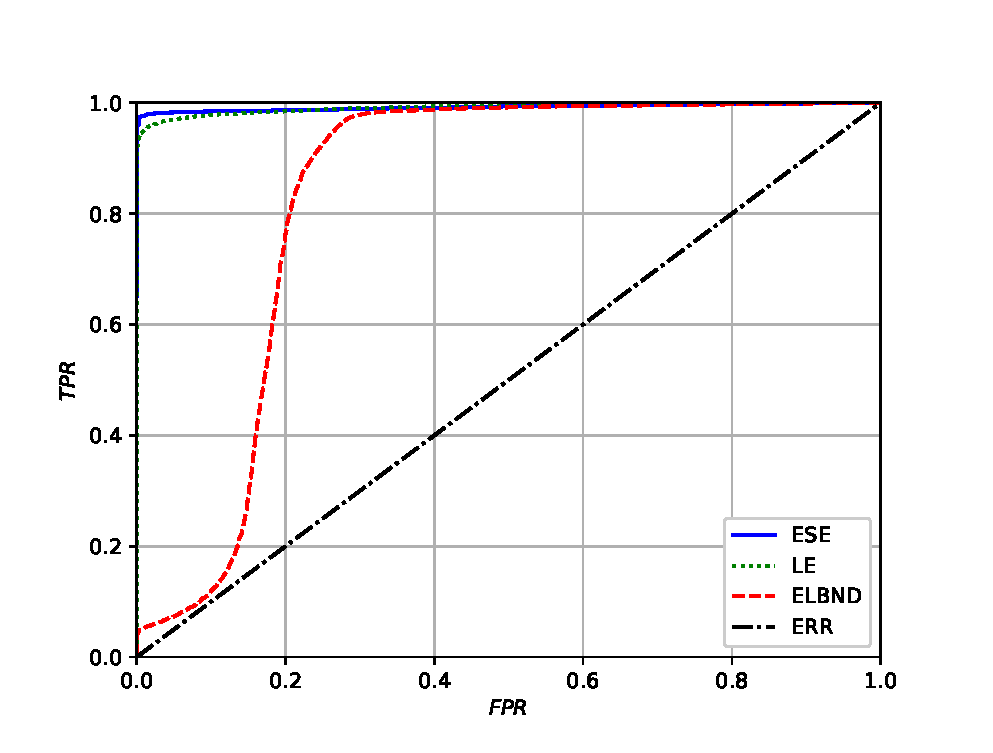
\includegraphics[scale=0.7]{IMG/appel_roc/roc_02.eps}
    \caption{ROC křivky v případě detekce změny trendu signálu obsahujícího aditivní gaussovský šum se směrodatnou odchylkou $\sigma_n=.2$. Průměrná hodnota $SNR$ experimentů byla $SNR=30.00$ $dB$. Černá čerchovaná čára (RANDOM) reprezentuje náhodný klasifikátor.}
    \label{fig:roc_02}
\end{figure}
\begin{figure}[ht!]
    \centering
    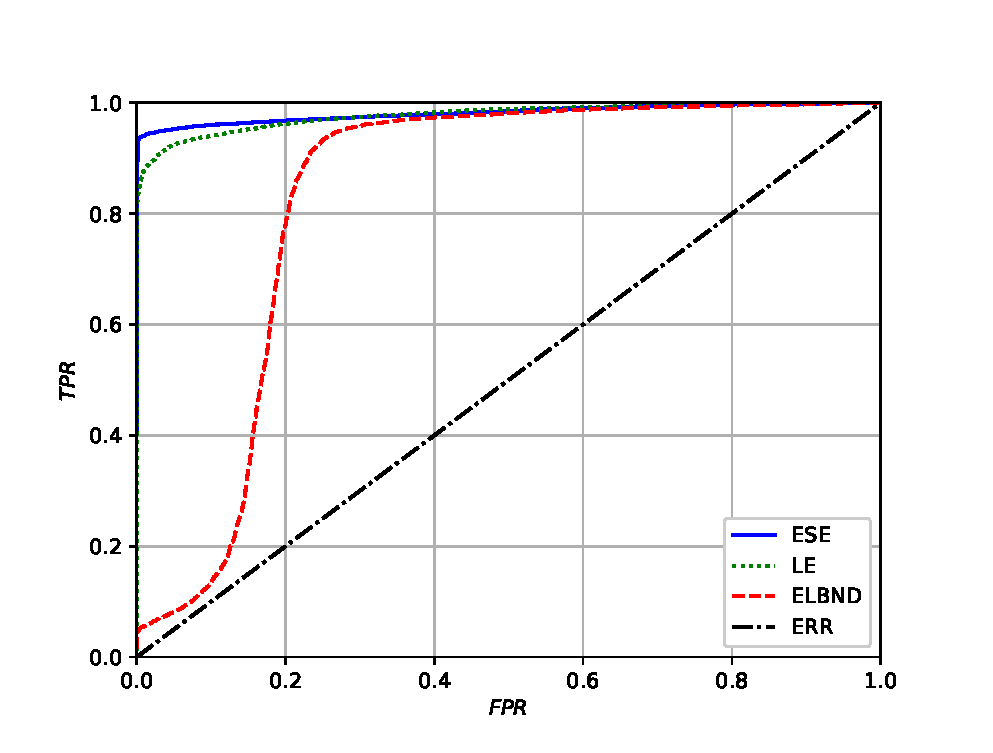
\includegraphics[scale=0.73]{IMG/appel_roc/roc_05.eps}
    \caption{ROC křivky v případě detekce změny trendu signálu obsahujícího aditivní gaussovský šum se směrodatnou odchylkou $\sigma_n=0.5$. Průměrná hodnota $SNR$ experimentů byla $SNR=21.70$ $dB$. Černá čerchovaná čára (RANDOM) reprezentuje náhodný klasifikátor.}
    \label{fig:roc_05}
\end{figure}
\begin{figure}[ht!]
    \centering
    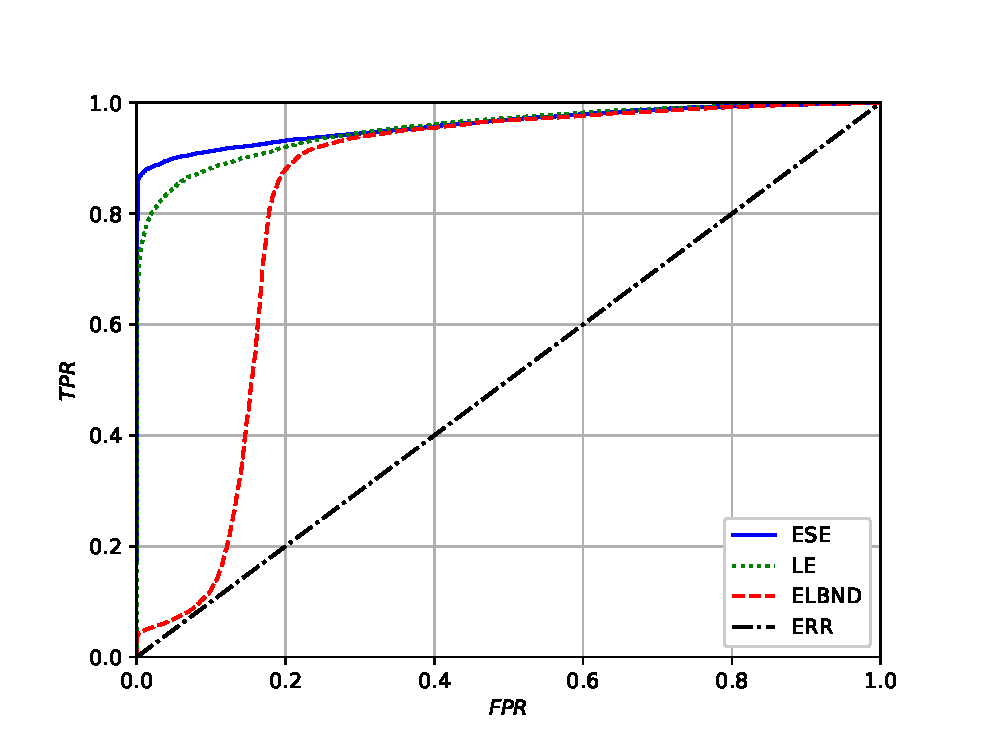
\includegraphics[scale=0.73]{IMG/appel_roc/roc_1.eps}
    \caption{ROC křivky v případě detekce změny trendu signálu obsahujícího aditivní gaussovský šum se směrodatnou odchylkou $\sigma_n=1.0$. Průměrná hodnota $SNR$ experimentů byla $SNR=16.20$ $dB$. Černá čerchovaná čára (RANDOM) reprezentuje náhodný klasifikátor.}
    \label{fig:roc_1}
\end{figure}
\begin{figure}[ht!]
    \centering
    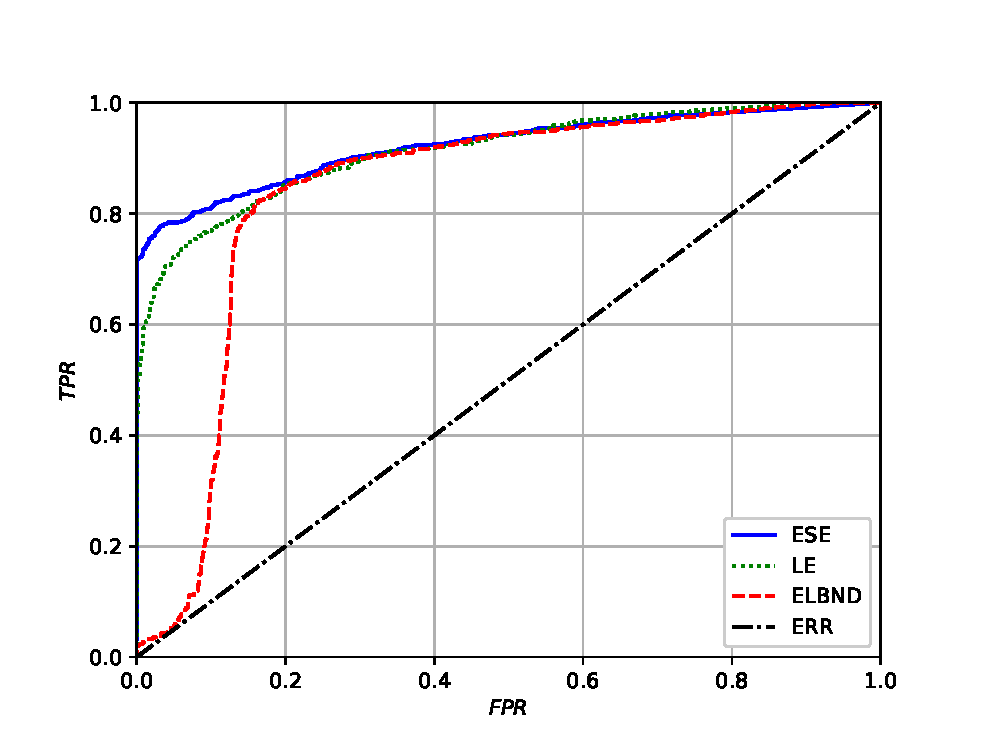
\includegraphics[scale=0.73]{IMG/appel_roc/roc_2.eps}
    \caption{ROC křivky v případě detekce změny trendu signálu obsahujícího aditivní gaussovský šum se směrodatnou odchylkou $\sigma_n=2.0$. Průměrná hodnota $SNR$ experimentů byla $SNR=10.88$ $dB$. Černá čerchovaná čára (RANDOM) reprezentuje náhodný klasifikátor.}
    \label{fig:roc_2}
\end{figure}
\begin{figure}[ht!]
    \centering
    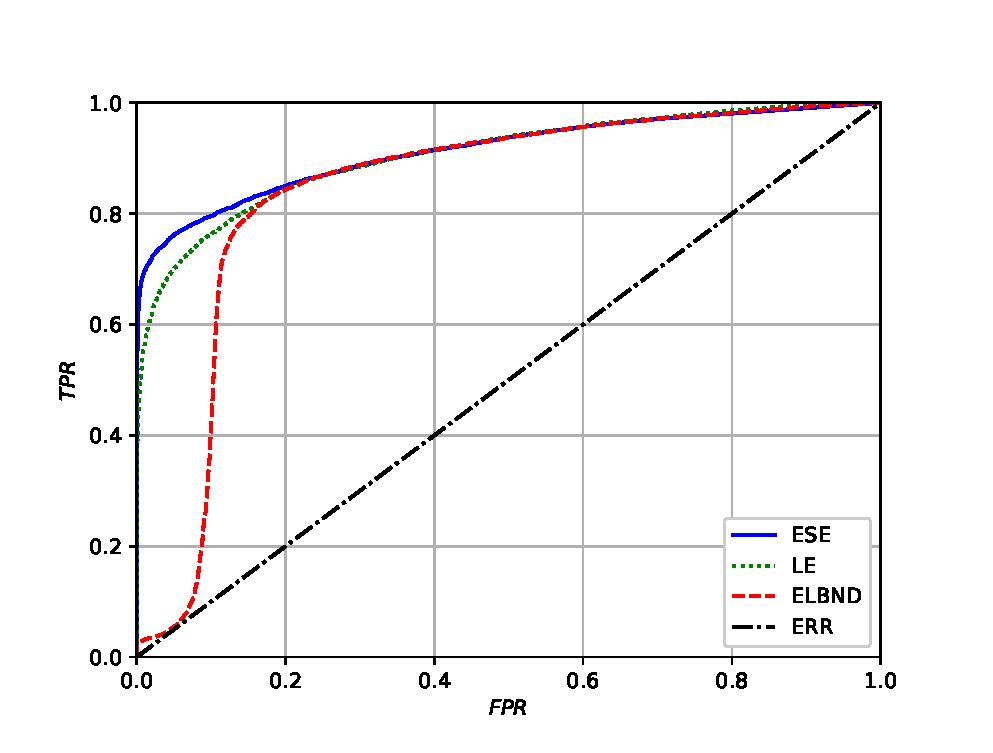
\includegraphics[scale=0.73]{IMG/appel_roc/roc_25.eps}
    \caption{ROC křivky v případě detekce změny trendu signálu obsahujícího aditivní gaussovský šum se směrodatnou odchylkou $\sigma_n=2.5$. Průměrná hodnota $SNR$ experimentů byla $SNR=9.20$ $dB$. Černá čerchovaná čára (RANDOM) reprezentuje náhodný klasifikátor.}
    \label{fig:roc_25}
\end{figure}

\section{Vyhodnocení výpočetní náročnosti metod odhadu parametrů zobecněného Paretova rozdělení}\label{chap:appel_gpd}
Výsledky v této podkapitole byli publikovány v \ref{appel2}. Cílem bylo určit výpočetní čas výpočtu parametrů GPD v typické aplikaci pro použití algoritmu ESE, který byl, v tomto případě, testován ne experimentu detekce skokové změny parametrů generátoru signálu.
\subsection{Motivace}
Detekce novosti v reálném čase je úloha, která nalézá své uplatnění nejen v oblasti detekci a diagnostiky v průmyslových aplikacích \cite{fault}, ale také např. v detekci narušení počítačových sítí \cite{data_streams} nebo v zabezpečovacích systémech \cite{surveilance}. Další oblastí uplatnění je např. mobilní robotika, která je specifická tím, že robot má k dispozici pouze limitovaný výpočetní výkon \cite{robotics_marslan,robotics}. Pro metody detekce novosti v reálném čase je tedy důležité, aby vynikali dostatečně nízkou výpočetní náročností. Z tohoto důvodu byli otestovány tři různé metody výpočtu parametrů GPD, protože tento výpočet je z hlediska použití algoritmu ESE potenciálně limitující z hlediska využitelnosti v aplikacích detekce v reálném čase. Jmenovitě byli otestovány tyto metody: metoda maximální věrohodnosti (ML), metoda momentů (MOM) a metoda kvazi-maximální věrohodnosti (QML). Výpočetní čas potřebný k určení parametrů GPD pomocí těchto metod byl vyhodnocen při experimentu, ve kterém dojde ke skokové změně parametrů generátoru signálu.
\subsection{Specifikace experimentu}
Vzhledem k povaze experimentu, který slouží k vyhodnocení výpočetní náročnosti různých metod určení parametrů GPD, a nikoliv k detekci novosti v nějakém komplexním procesu, byl zvolen jednoduchý lineární kombinační filtr (LNU), jehož výstup v diskrétním časovém okamžiku $k$ je definován jako
\begin{equation}\label{eq:gene_ese_1}
\hat{y}(k)=w_1\cdot x_1(k)+w_2\cdot x_2(k)+w_3\cdot x_3(k)
\end{equation}
a tento filtr je adaptován algoritmem NLMS.
\par 
Pro výstup generátoru signálu platí vztah
\begin{equation}
y(k)=x_1(k)+x_2(k)+x_3(k)+v(k)
\end{equation}
pro všechny $1 \leq k \leq 200$. Člen $v(k)$ reprezentuje aditivní gaussovský šum s nulovou střední hodnotou a směrodatnou odchylkou $\sigma_{noise}=0.1$. V diskrétním časovém okamžiku $k=201$ dojde ke změně generátoru signálu a jeho výstup přejde do tvaru
\begin{equation}
y(k)=0.7\cdot x_1(k)+1.2\cdot x_1(k)+1.1 \cdot x_1(k) + v(k)
\end{equation}
pro $201 \leq k \leq 400$. Hodnota všech vstupů generátoru signálu je v každém časovém okamžiku $k$ vybrána ze standartního rozdělení normálního rozdělení, takže $i$-tý vstup $x_i\sim \mathcal{N}(0,1)$. Změna parametrů signálu byla vybrána tak, aby nedošlo ke změně střední hodnoty signálu $y(k)$.
\par
Délka okna pro odhad parametrů GPD byla během experimentu nastavena na $n_s=1200$. Před experimentem bylo pořízení 1200 vzorků vygenerovaných generátorem signálu definovaným vztahem \ref{eq:gene_ese_1}, na něž byla použita metoda POT, tak aby při experimentu v diskrétní časový okamžik $k=1$ byla hodnota ESE relevantní.
\par
Průběh výstupní hodnoty filtru je zobrazen na obrázku \ref{fig:par_output}, hodnota ESE potom na obrázku \ref{fig:par_ese}. Hodnoty parametrů $\xi$, $\sigma$, $\mu$ GPD, pro všechny tři adaptivní váhy, během experimentu jsou zobrazeny na obrázcích \ref{fig:par_gamma}, \ref{fig:par_sigma} a \ref{fig:par_mu}.
\par
Experiment byl proveden na PC s procesorem Intel(R) Core(TM) i5-7400 se 4mi jádry s taktovací frekvencí 3001 MHz a operační pamětí o velikosti 32 GB. Operační systém byl Windows 10 Pro, 64-bitová verze 10.0.18362. Kód byl napsán v Python 3.6.1 \cite{python} a byly použity knihovny Numpy 1.17.0 \cite{numpy} a Scipy 1.4.1 \cite{scipy}.


\begin{figure}[h!]

	\centering
	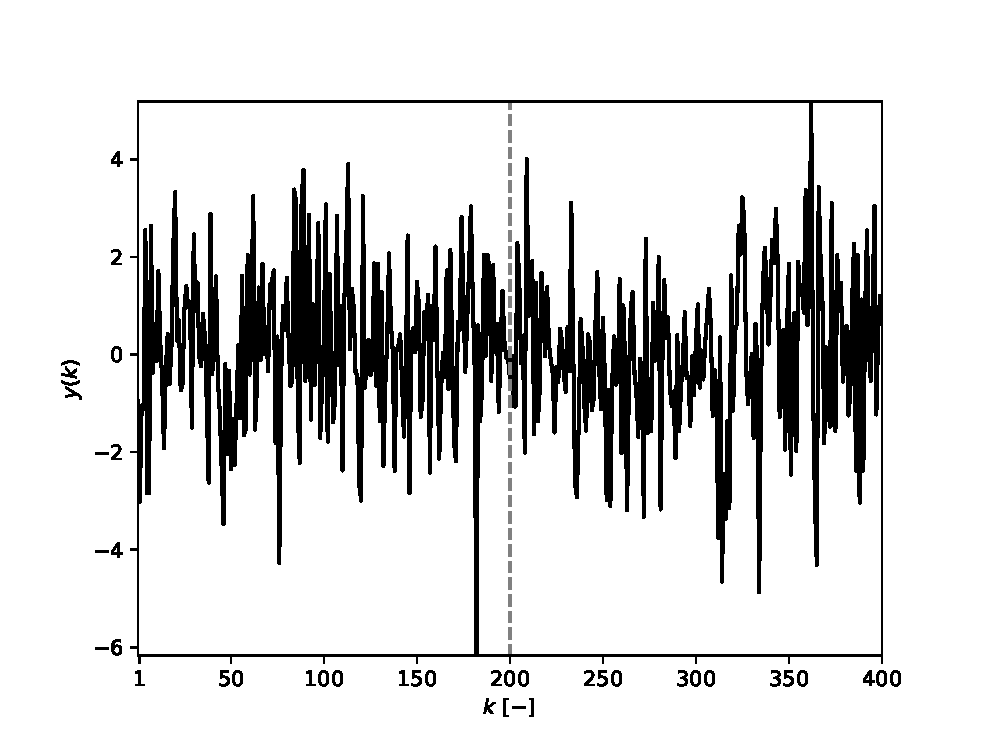
\includegraphics[scale=0.74]{IMG/appel_par/par_output.eps}
	\caption{Výstup adaptivního filtru během experimentu. Skoková změna parametrů generátoru signálu je zvýrazněná svislou vodorovnou čarou v diskrétním časovém okamžiku $k=200$.}
		\label{fig:par_output}
\end{figure}

\subsection{Výsledky a diskuze}


\begin{figure}[h!]

	\centering
	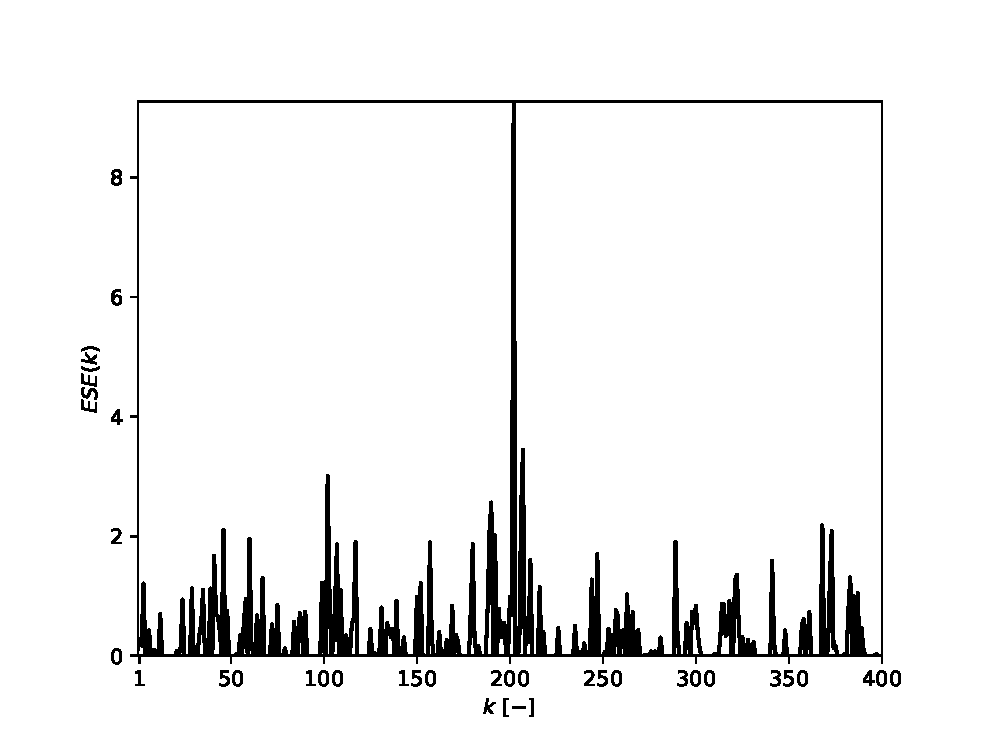
\includegraphics[scale=0.74]{IMG/appel_par/par_ese.eps}
	\caption{Hodnota ESE během experimentu. Globální maximum odpovídá změně parametrů generátoru signálu, resp. úspěšné detekci novosti.}
		\label{fig:par_ese}
\end{figure}

\begin{figure}[h!]

	\centering
	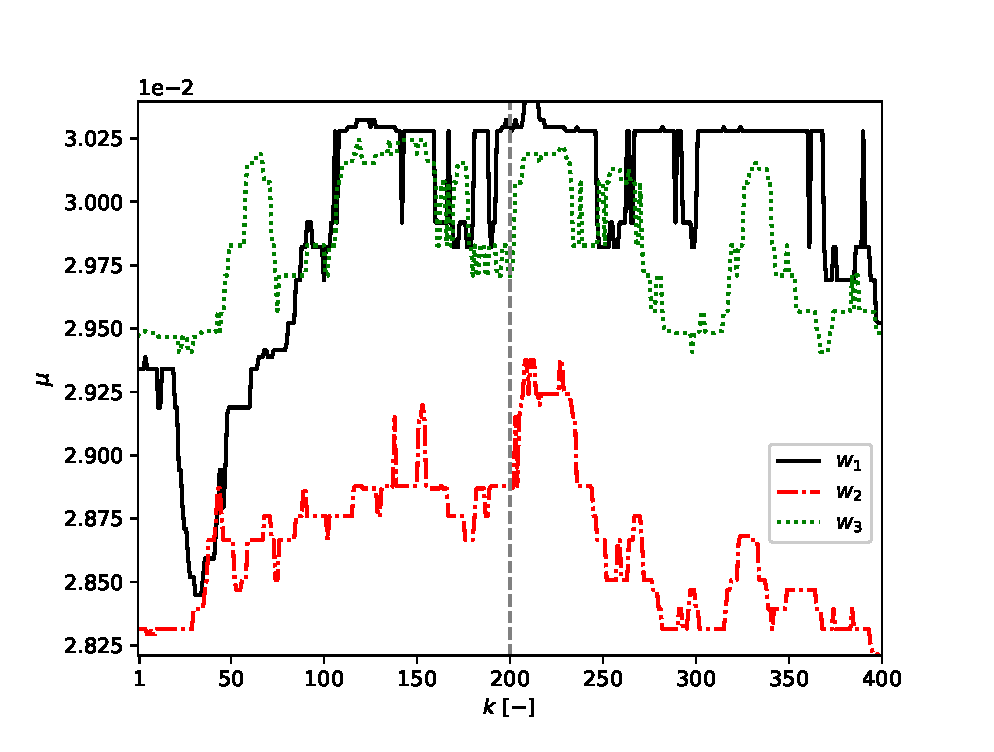
\includegraphics[scale=0.71]{IMG/appel_par/par_mu.eps}
	\caption{Hodnota parametru $\mu$ GPD pro všechny tři adaptivní váhy $w_1$, $w_2$, $w_3$ během experimentu detekce změn parametrů generátoru signálu. Svislá čára v diskrétním časovém okamžiku $k=200$ znázorňuje skokovou změnu parametrů generátoru signálu.}
		\label{fig:par_mu}
\end{figure}

\begin{figure}[h!]

	\centering
	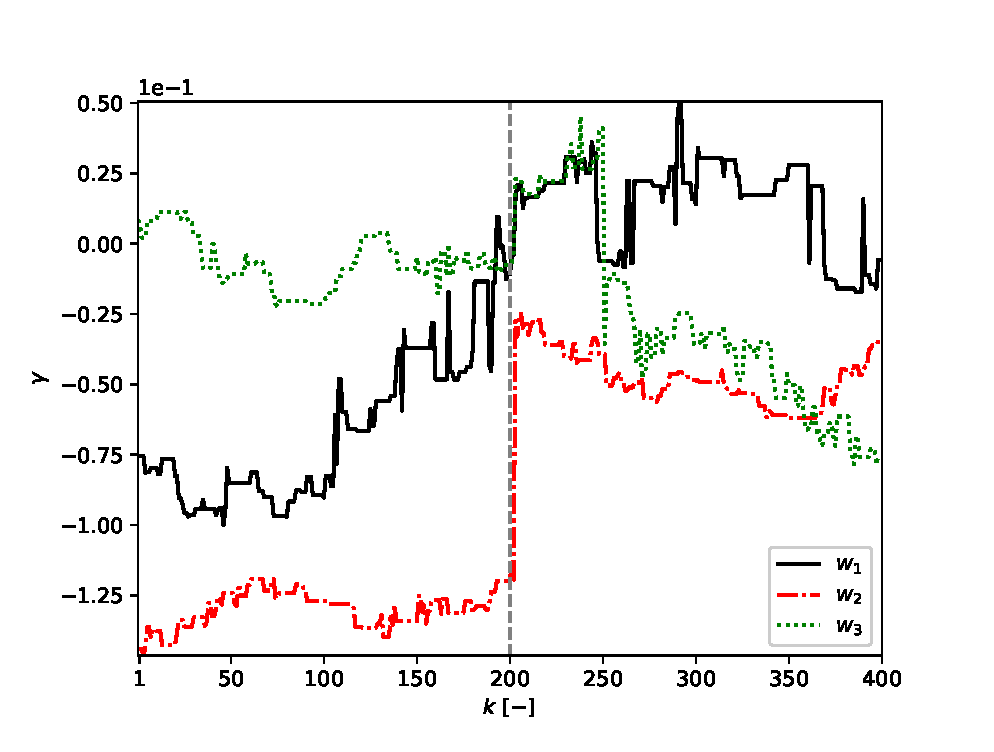
\includegraphics[scale=0.71]{IMG/appel_par/par_gamma.eps}
	\caption{Hodnota parametru $\gamma$ GPD pro všechny tři adaptivní váhy $w_1$, $w_2$, $w_3$ během experimentu detekce změn parametrů generátoru signálu. Svislá čára v diskrétním časovém okamžiku $k=200$ znázorňuje skokovou změnu parametrů generátoru signálu.}
		\label{fig:par_gamma}
\end{figure}

\begin{figure}[h!]

	\centering
	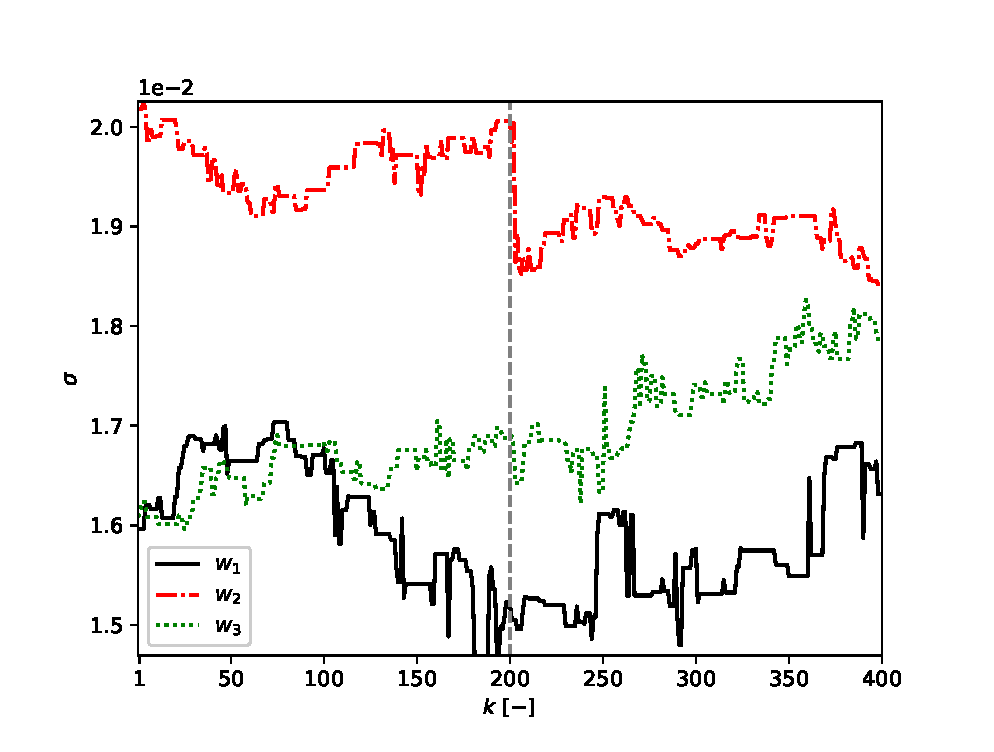
\includegraphics[scale=0.71]{IMG/appel_par/par_sigma.eps}
	\caption{Hodnota parametru $\sigma$ GPD pro všechny tři adaptivní váhy $w_1$, $w_2$, $w_3$ během experimentu detekce změn parametrů generátoru signálu. Svislá čára v diskrétním časovém okamžiku $k=200$ znázorňuje skokovou změnu parametrů generátoru signálu.}
		\label{fig:par_sigma}
\end{figure}
Průměrný čas výpočtu $\overline{t}$ parametrů všech tří GPD (počet GPD odpovídá počtu adaptivních parametrů filtru) a odpovídající směrodatné odchylky $\sigma_t$ jsou uvedeny v následující tabulce \ref{tab:par_results}. Čas výpočtu je určený pro jeden experiment (400 vzorků).
\begin{table}[h!]

\centering
\caption{Tabulka průměrných časů výpočtu pro jednotlivé adaptivní váhy a odpovídajících směrodatných odchylek vybraných metod výpočtu parametrů GPD}
\begin{tabular}{|l|l||l|l|}
\hline
 & Metoda & $\overline{t}$ {[}ms{]} & $\sigma_t$ {[}ms{]} \\ \hline \hline
\multirow{3}{*}{$w_1$} & ML & $26.198$ & $3.396$ \\ \cline{2-4} 
 & QML & $0.354$ & $0.478$ \\ \cline{2-4} 
 & MOM & $\textbf{0.076}$ & $0.264$ \\ \hline
\multirow{3}{*}{$w_2$} & ML & $26.718$ & $2.302$ \\ \cline{2-4} 
 & QML & $0.337$ & $0.471$ \\ \cline{2-4} 
 & MOM & $\textbf{0.064}$ & $0.244$ \\ \hline
\multirow{3}{*}{$w_3$} & ML & $24.982$ & $1.964$ \\ \cline{2-4} 
 & QML & $0.395$ & $0.489$ \\ \cline{2-4} 
 & MOM & $\textbf{0.060}$ & $0.238$ \\ \hline

\end{tabular}
 \label{tab:par_results}
\end{table}

Z uvedených výsledků je patrné, že nejrychlejší metoda je MOM. Podstatnou nevýhodou této metody pro využití v aplikacích, které vyhodnocují data v reálném čase je její omezení na hodnoty parametrů GPD. Pokud parametry uvedené omezení nesplňují, vypočtené hodnoty nepřesné (resp. nesmyslné) a tedy nepoužitelné pro algoritmus ESE, který začne produkovat nepřesné výsledky. Z pohledu úlohy detekce novosti je diskutabilní, zda-li můžeme garantovat, že sledovaný proces po celou dobu bude splňovat uvedené omezení.
\par
Metoda, jejíž výpočetní čas byl nejvyšší je ML, což je vzhledem k iterativnímu určení parametrů GPD očekávatelné. Nevýhoda použití této metody tkví v  nemožnosti určit minimální resp. maximální počet iterací. Jednou z možností jak zrychlit nalezení parametrů je využití apriorní informace o hodnotách těchto parametrů. V rámci experimentu však byla využita pouze apriorní informace o parametru $\mu$, který odpovídá nejmenší hodnotě přírůstku vah, které byli získány metodou POT aplikovanou na plovoucí okno délky $n_s$.
\par
Dobrým kompromisem mezi výše uvedenými metodami je použití metody QML. Výpočetní čas této metody byl v uvedeném experimentu o dva řády kratší než ML a asi pětkrát delší než MOM. Pro každou z vyhodnocovaných vah byl kratší než $500$ $\mu s$.
\par 
Z provedeného experimentu je patrné, že použití algoritmu ESE pro aplikace v reálném čase je limitováno počtem parametrů filtru a rychlostí vzorkování monitorovaného procesu. 







 
\chapter{Závěr}
Předložená dizertační práce je věnována použití adaptivních systémů při analýze dat. Za zásadní výsledek lze považovat nový originální algoritmus pro detekci novosti, který vyhodnocuje přírůstky adaptivních vah filtru, Extreme Seeking Entropy \ref{ese_mdpi} (viz kapitola \ref{chap:ese}). Tento algoritmus byl otestován v následujících případových studiích (viz kapitola \ref{chap:vysledky}): detekce pertubace v chaotické časové řadě získané řešením Mackey-Glassovy rovnice, detekce změny rozptylu šumu v náhodném datovém toku, detekce skokové změny parametrů generátoru signálu, detekce náhlé absence šumu, detekce změny trendu a při detekci epilepsie v myším EEG. Pro detekci skokové změny trendu a skokové změny parametrů signálu byla vyhodnocena úspěšnost této detekce a výsledky porovnány s výsledky algoritmů Learning Entropy a Error and Learning Based Novelty Detection, přičemž v obou případech byla úspěšnost detekce algoritmu ESE vyšší pro téměř všechny vyhodnocované hodnoty SNR. Pro hodnotu $SNR>34$ $dB$ dosáhl algoritmus při detekci skokové změny parametrů generátoru signálu $100\%$ úspěšnost. Při detekci změny trendu měl algoritmus ESE pro hodnoty $SNR>8$ $dB$ větší úspěšnost detekce než srovnávané algoritmy LE a ELBND. Výše uvedené výsledky byly publikovány v \ref{ese_mdpi}.
\par Pro možné použití v aplikacích detekce v reálném čase byla experimentálně zjišťována výpočetní časová náročnost různých metod odhadů parametrů zobecněného Paretova rozdělení v případě použití algoritmu ESE při detekci skokové změny parametrů \ref{appel2}. Výsledkem je porovnání 3 různých metod odhadu parametrů. Limitujícím faktorem použití ESE v reálném čase je v zásadě počet adaptivních parametrů filtru, které je potřeba vyhodnocovat a samozřejmě rychlost vzorkování monitorovaného signálu.
\par Pro odhad úspěšnosti detekce novosti pomocí algoritmu ESE byla také vyhodnocena ROC křivka v případě detekce změny trendu signálu s různými poměry SNR a byly určeny příslušné plochy pod těmito ROC křivkami \ref{appel3}. Dosažené výsledky byly opět porovnány s algoritmy LE a ELBND a bylo ověřeno, že pro hodnoty $SNR \leq 30$ $dB$ dosahuje algoritmus ESE lepších výsledků. Pro vyšší hodnoty $SNR$ pak byly výsledky ESE srovnatelné s výsledky LE.  Cílem této studie bylo zjistit jak dobře dokáže algoritmus ESE separovat nová data v závislosti na volbě prahu, který rozhoduje o tom zda data obsahují novost či nikoliv. Pro představu ještě uveďme, že např. pro hodnotu $SNR=16.2$ $dB$ bylo dosaženo úspěšnosti detekce $90.42\%$.
\par
Stanovené cíle dizertační práce (viz kapitola \ref{chap:cile}) tak lze, na základě výše uvedených výsledků, považovat za splněné.

\section{Možné směry budoucího výzkumu}
V budoucnu se nabízí rozvíjet téma využití adaptivních systémů ve zpracování dat několika směry. Potenciální využití vyhodnocení změn vah adaptivních systémů lze využít v optimalizaci velikosti datasetů v oblasti hlubokého učení, což by mohlo výrazně snížit časovou náročnost učení hlubokých sítí. Za účelem snížení výpočetního času algoritmu ESE je potřeba vyzkoušet další metody odhadu parametrů zobecněného Paretova rozdělení a vyzkoušet adaptivní metody volby velikosti prahu pro metodu Peak-over-threshold. Zajímavým tématem je také vliv šumu a jeho typu na velikost přírůstků adaptivních vah filtrů a jejich pravděpodobnostní rozdělení. V neposlední řadě se nabízí otázka, jak ovlivní typ kriteriální funkce pro optimalizaci adaptivního filtru výsledky algoritmu ESE a je-li možné různé kriteriální funkce využívat k detekci novosti, případně pomocí nich typ novosti klasifikovat. 

\renewcommand{\bibname}{Publikace autora}
\begin{thebibliography}{A}
\end{thebibliography}

\begin{enumerate}[label={[V\arabic*]}]
    \item \label{ese_mdpi} VRBA, Jan; MAREŠ, Jan. Introduction to Extreme Seeking Entropy. \textit{Entropy}, 2020, 22.1: 93.
  	\item \label{appel2}VRBA, Jan; MAREŠ, Jan. Computational Performance of the Parameters Estimation in Extreme Seeking Entropy Algorithm. In: \textit{2020 International Conference on Applied Electronics (AE)}. IEEE, 2020. p. 1-4.
	\item \label{appel3}VRBA, Jan; MAREŠ, Jan. ROC Analysis of Extreme Seeking Entropy for Trend Change Detection. In: \textit{2020 International Conference on Applied Electronics (AE)}. IEEE, 2020. p. 1-4.  
	\item \label{artep}VRBA, Jan. Využití fuzzy systémů a algoritmu learning entropy pro detekci změn stavů bioprocesu. In: \textit{Automatizacia a riadenie v teorii a praxi ARTEP 2017}. Technická univerzita Košice, 2017.

	\item \label{asr} VRBA, Jan. \textit{XLIII. Seminář ASŘ - Adaptivní metoda detekce} [přednáška]. Ostrava: VŠB TU Ostrava, 27.4.2018.
    \item \label{appel1}VRBA, Jan. Adaptive Novelty Detection with Generalized Extreme Value Distribution. In: \textit{2018 International Conference on Applied Electronics (AE)}. IEEE, 2018. p. 1-4.
    \item \label{ijcnn}BUKOVSKÝ, Ivo, et al. Study of learning entropy for onset detection of epileptic seizures in EEG time series. In: \textit{2016 International Joint Conference on Neural Networks (IJCNN)}. IEEE, 2016. p. 3302-3305.

    
    \item \label{cyril}OSWALD, Cyril, et al. Novelty Detection in System Monitoring and Control with HONU. In: \textit{Applied Artificial Higher Order Neural Networks for Control and Recognition}. IGI Global, 2016. p. 61-78.


	\item \label{roboti}VRBA, Jan, et al. An Automated Platform for Microrobot Manipulation. In: \textit{International Workshop on Soft Computing Models in Industrial and Environmental Applications}. Springer, Cham, 2020. p. 255-265.
	\item \label{bila1}BÍLA, Jiří; VRBA, Jan. The Detection and Interpretation of Emergent Situations in ECG Signals. In: \textit{International Conference on Soft Computing-MENDEL}. Springer, Cham, 2016. p. 264-275.

	\item \label{ijcnn3}MOJZES, Matej, et al. Feature selection via competitive levy flights. In: \textit{2016 International Joint Conference on Neural Networks (IJCNN)}. IEEE, 2016. p. 3731-3736.
	
	\item \label{bila2}BÍLA, Jiří; NOVÁK, Martin; VRBA, Jan. Detection of emergent situations in complex systems represented by algebras of transformations. In: \textit{MATEC Web of Conferences}. EDP Sciences, 2016. p. 02035.	
	\item \label{artep2}BUKOVSKÝ, Ivo, OSWALD, Cyril, VRBA, Jan. Případová studie použití entropie učení pro adaptivní detekci při řízení spalování tuhých paliv. In: \textit{Automatizácia a riadenie v teórii a praxi 2015}. Technická univerzita Košice, 2015.
\end{enumerate}

\renewcommand{\bibname}{Literatura relevantní k tezím}
\begin{thebibliography}{L}
\bibitem{expo}SHARMA, Anish and ANDREWS, Rebecca. Managing-Exponential-Data-Growth-and-Application-Modernization. \textit{IBM} [online]. 11 November 1999. [cit. 11.8.2020]. Dostupné z: https://www.ibm.com/cloud/blog/managing-exponential-data-growth-and-application-modernization 
\bibitem{ivoLE1}BUKOVSKY, Ivo. Learning entropy: Multiscale measure for incremental learning. \textit{Entropy}, 2013, 15.10: 4159-4187.
\bibitem{ivoLE2}BUKOVSKY, Ivo; KINSNER, Witold; HOMMA, Noriyasu. Learning Entropy as a Learning-Based Information Concept. \textit{Entropy}, 2019, 21.2: 166.
\bibitem{elbnd1}CEJNEK, Matous; BUKOVSKY, Ivo. Concept drift robust adaptive novelty detection for data streams. \textit{Neurocomputing}, 2018, 309: 46-53.
\bibitem{elbnd2} CEJNEK, Matous; BUKOVSKY, Ivo. Influence of type and level of noise on the performance of an adaptive novelty detector. In: \textit{2017 IEEE 16th International Conference on Cognitive Informatics \& Cognitive Computing (ICCI* CC)}. IEEE, 2017. p. 373-377.
\bibitem{elbnd3}CEJNEK, Matous; BUKOVSKY, Ivo; VYSATA, Oldrich. Adaptive classification of EEG for dementia diagnosis. In: \textit{2015 International Workshop on Computational Intelligence for Multimedia Understanding (IWCIM)}. IEEE, 2015. p. 1-5.
\bibitem{mackey}MACKEY, Michael C.; GLASS, Leon. Oscillation and chaos in physiological control systems. \textit{Science}, 1977, 197.4300: 287-289.
\bibitem{dead}SPANGENBERG, Mariana, et al. Detection of variance changes and mean value jumps in measurement noise for multipath mitigation in urban navigation. \textit{Navigation}, 2010, 57.1: 35-52.
\bibitem{stepchange}L'ECUYER, Pierre. History of uniform random number generation. In: \textit{2017 Winter Simulation Conference (WSC)}. IEEE, 2017. p. 202-230.
\bibitem{diagnosis}MAURYA, Mano Ram; RENGASWAMY, Raghunathan; VENKATASUBRAMANIAN, Venkat. Fault diagnosis using dynamic trend analysis: A review and recent developments. \textit{Engineering Applications of artificial intelligence}, 2007, 20.2: 133-146.
\bibitem{roc_orig}EGAN, James P. \textit{Signal detection theory and ROC-analysis}. Academic press, 1975.
\bibitem{roc_bible}FAWCETT, Tom. An introduction to ROC analysis. \textit{Pattern recognition letters}, 2006, 27.8: 861-874.
\bibitem{fault}GERTLER, Janos. \textit{Fault detection and diagnosis in engineering systems}. CRC press, 1998.
\bibitem{data_streams}YU, Kangqing, et al. Real-time Outlier Detection over Streaming Data. In: \textit{2019 IEEE SmartWorld, Ubiquitous Intelligence \& Computing, Advanced \& Trusted Computing, Scalable Computing \& Communications, Cloud \& Big Data Computing, Internet of People and Smart City Innovation (SmartWorld/SCALCOM/UIC/ATC/CBDCom/IOP/SCI)}. IEEE, 2019. p. 125-132.
\bibitem{surveilance}
RAMEZANI, Ramin; ANGELOV, Plamen; ZHOU, Xiaowei. A fast approach to novelty detection in video streams using recursive density estimation. In: \textit{2008 4th International IEEE Conference Intelligent Systems. IEEE, 2008}. p. 14-2-14-7.
\bibitem{robotics_marslan}
MARSLAND, Stephen; NEHMZOW, Ulrich; SHAPIRO, Jonathan. On-line novelty detection for autonomous mobile robots. \textit{Robotics and Autonomous Systems}, 2005, 51.2-3: 191-206.
\bibitem{robotics}
NEHMZOW, Ulrich, et al. Novelty detection as an intrinsic motivation for cumulative learning robots. In: \textit{Intrinsically Motivated Learning in Natural and Artificial Systems}. Springer, Berlin, Heidelberg, 2013. p. 185-207.
\bibitem{python}VAN ROSUM, G.; DRAKE, F. L. \textit{Python 3 Reference Manual}. Scotts Valley, CA: CreateSpace, 2009.
\bibitem{numpy}OLIPHANT, Travis E. \textit{A guide to NumPy (Vol. 1)}. Trelgol Publishing USA, 2006.
\bibitem{scipy}VIRTANEN, P. et al.  SciPy 1.0: Fundamental Algorithms for Scientific Computing in Python. \textit{Nature Methods}, 2020, 17(3), 261-272.
\end{thebibliography}
\cleardoublepage
\thispagestyle{empty}\

\newpage
\end{document}